% Plain-language review document (explaneat plain-language review), v5.
\documentclass[a4paper,10pt]{article}
\usepackage[margin=1.8cm]{geometry}
\usepackage{amsmath}
\usepackage{amssymb}
\usepackage{booktabs}
\usepackage{tabularx}
\usepackage{graphicx}
\usepackage[table,usenames,dvipsnames]{xcolor}
\usepackage{tikz}
\usetikzlibrary{arrows.meta,fit,backgrounds,positioning,calc}
\usetikzlibrary{shapes.geometric}
\usepackage{longtable}
\usepackage{pdflscape}
\usepackage{float}
\usepackage[font=small,labelfont=bf]{caption}
\usepackage{array}
\usepackage[unicode=true,hidelinks]{hyperref}
\setcounter{tocdepth}{3}
\setcounter{secnumdepth}{3}
% Review markers, copied from dissertation.tex (7 Nov 2026) for standalone builds.
\newif\ifreviewmarks
\reviewmarkstrue
\newcommand{\reviewrule}{\noindent{\color{BrickRed}\rule{\linewidth}{0.8pt}}}
\newenvironment{drafted}[1][]{%
  \ifreviewmarks\par\addvspace{\medskipamount}\reviewrule\par\nopagebreak
  \noindent{\color{BrickRed}\sffamily\footnotesize\textbf{Thesis Draft}\quad #1\hfill review}\par\nopagebreak\smallskip\fi}{%
  \ifreviewmarks\par\smallskip\noindent{\color{BrickRed}\sffamily\footnotesize end of thesis draft}\par\nopagebreak\reviewrule\par\medskip\fi}
\newcommand{\figreview}[1]{\ifreviewmarks\par\smallskip{\color{NavyBlue}\sffamily\footnotesize\textbf{Figure note:} #1}\par\fi}
\begin{document}
\begin{center}{\Large\bfseries Plain-language explanation: heart-s4-c1\par}\vspace{2mm}{\small AI-assisted drafts for review. Nothing here has been verified by a person.\par}\end{center}
\noindent\textbf{How to read this.} Explanations are built up but read down: the summary first, then each part from the whole model down, in plain words, each sentence followed by the claims it rests on (C01, C02, \ldots; every cited claim was computed on the model and checked). Numbers are changes in predicted risk for a typical patient. The technical record (original hypotheses, formulas, evidence tables with the test check, ranges and n) is at the end. The text describes what the model does, not the world; whether it is plausible is for the reviewer to judge.
\par\medskip\noindent\textbf{What changed in v5e (figures).} v5e: every diagram is a numbered figure with a caption (list of figures after the contents) and the text refers to it; the whole-network figure has its own landscape page, scaled to the page, with a short caption and its description in the text; an input used by several parts is drawn under each of them (same input, repeated for readability, dotted outline); and an appendix figure shows the trained network before any explanation (no parts, no splits).
\par\medskip\noindent\textbf{What changed in v5c (tables and diagrams).} v5c: the evidence tables are landscape, compact and shaded by row, with the header repeated on every page (longtable and pdflscape, used in this review PDF only; the thesis preamble has neither). In the diagrams each input is drawn once, in a shared row along the bottom (the explanation's split copies of an input are listed in the technical detail instead), every cluster has one output rectangle with its plain name, the inputs that feed the output directly meet in a drawn 'sum', and a one-line legend explains the edges.
\par\medskip\noindent\textbf{What changed in v5b (diagrams).} v5b uses one grouping everywhere, the annotation hierarchy: the summary's diagram is the same picture as the whole model's section, and a part that is itself a weighted sum (blood pressure with cholesterol) is a part of its own, described as one that adds up, so the text counts three parts throughout; the lint checks every 'N parts' against the hierarchy. A full-structure diagram follows the summary: every node and connection, nested by part, with the inputs that feed the output directly in their own cluster and the unused input columns listed. Each section from the top down adds its own region of that diagram, with stubs for connections from or to other parts; each connection is drawn in exactly one section. The gate's text now says that it lowers the risk for the patients it acts on, and that more vessels and higher cholesterol take that lowering away; its vessel statements are one per group.
\par\medskip\noindent\textbf{What changed in v5 (read down).} v5 reads the explanation down. The summary (one line, a diagram, one paragraph per block) is as in v4, except that the paragraph on what adds up is split into protective items, risk-raising items and rare results, and an input that also feeds a part is quoted with its direct contribution only (the rest is in that part's paragraph). Then the document walks the annotation hierarchy from the whole model down: for each part a plain hypothesis (what it does for the prediction), plain evidence (what was checked and what it showed; for a part made of others, what they are and how they combine), a diagram one level down and where to read on. The original hypotheses, closed forms and evidence tables are in 'Technical detail' at the end. Statements about structure (what a part is made of, a copy of another part, a formula that reproduces it) are now claims of their own, checked on the graph and the data.
\par\medskip\noindent\textbf{v4.} v4 follows the structure of the explanation. The summary opens with one line and a diagram at the same grouping, then gives one paragraph per top-level block of the annotation hierarchy: one for everything that adds up independently (the inputs that feed the model score directly, and parts that are a weighted sum), and one for each part that combines its inputs in another way: what it combines, how, and for whom. 'Parts in detail' follows the hierarchy below that, with a diagram one level down for each part that contains others. The prose no longer says 'clearly', 'slightly', 'consistently' or 'on the training data only': the numbers carry it, and the test check, the ranges and n stay in the evidence tables. Only genuinely small groups are marked, with their n. The lint rejects the confidence words and checks the block structure.
\tableofcontents
\listoffigures
\clearpage
\begin{drafted}[plain-language layer: heart-s4-c1]
\section{heart-s4-c1}
\noindent{\small Genome \texttt{c85804fa-08bd-4207-ac69-a31a8567473c}, explanation \texttt{10565a81-f55b-47f4-b51e-21641ec08556}. Split: train primary (n=242), test as a check (n=61). Claims: 47, verified 45, not supported 2.\par}
\noindent{\small\textcolor{BrickRed}{AI-assisted draft for review (unverified)}\par}\smallskip
\noindent{\footnotesize Reference (typical) patient: the typical patient: the median training patient for every number and the most common training category for every category (not a real patient). age: 56 years; ca: 0 vessels; chol: 240 mg/dL (6.2 mmol/L); cp: no chest pain (asymptomatic); exang: no chest pain on exercise; fbs: fasting blood sugar of 120 mg/dL or less; oldpeak: 0.8 mm; restecg: a normal resting ECG; sex: male; slope: an upsloping ST segment; thal: a normal thallium scan; thalach: 152 beats per minute; trestbps: 130 mm Hg. Predicted risk of heart disease: 24\%.\par}
\subsection{Summary}
\noindent For a typical patient (a 56-year-old man with no chest pain symptoms and median test results) the model predicts a risk of heart disease of about 24\%; it adds up most of its inputs independently, and four small parts add to that sum: one for a fixed defect on the thallium scan with normal fasting blood sugar, one for chest pain type, one for a downsloping ST segment and one for maximum heart rate.\,{\scriptsize\textcolor{NavyBlue}{[C31]}} Figure~\ref{fig:hearts4c1:summary} shows the model at this level: one box per paragraph below.
\par\medskip\noindent\fbox{\begin{minipage}{0.96\linewidth}\small\textbf{How to read the diagrams.} Edge colour is the sign of that one connection: blue positive, red negative; thicker is a larger weight. The outline and arrow on an input (and on a part's output box) is its overall effect on the final prediction, read from the verified claims: orange and up arrow raises it, teal and down arrow lowers it, grey and double arrow depends (it goes both ways, or differs between levels). A negative connection into a part that itself raises the prediction means that input lowers the prediction; through a hinge the overall effect can only be read from the claims, not from the edges. Up arrow means towards heart disease; down arrow, away from it. A double outline marks an input (or a part's output) that acts at a fixed rate everywhere: it adds the same amount to the score per unit, so it is explained by its rate alone (see 'Linear factors'); a dashed double outline, at a fixed rate on the observed data. The normal outline is an input whose effect switches on and off somewhere. For example, no chest pain has a negative connection into 'Chest pain offset', a part that lowers the predicted risk of heart disease, so no chest pain raises it.\end{minipage}}\par\medskip
\begin{figure}[H]\centering
\resizebox{!}{\ifdim\height>0.5\textheight 0.5\textheight\else\height\fi}{%
\resizebox{\ifdim\width>\linewidth\linewidth\else\width\fi}{!}{%
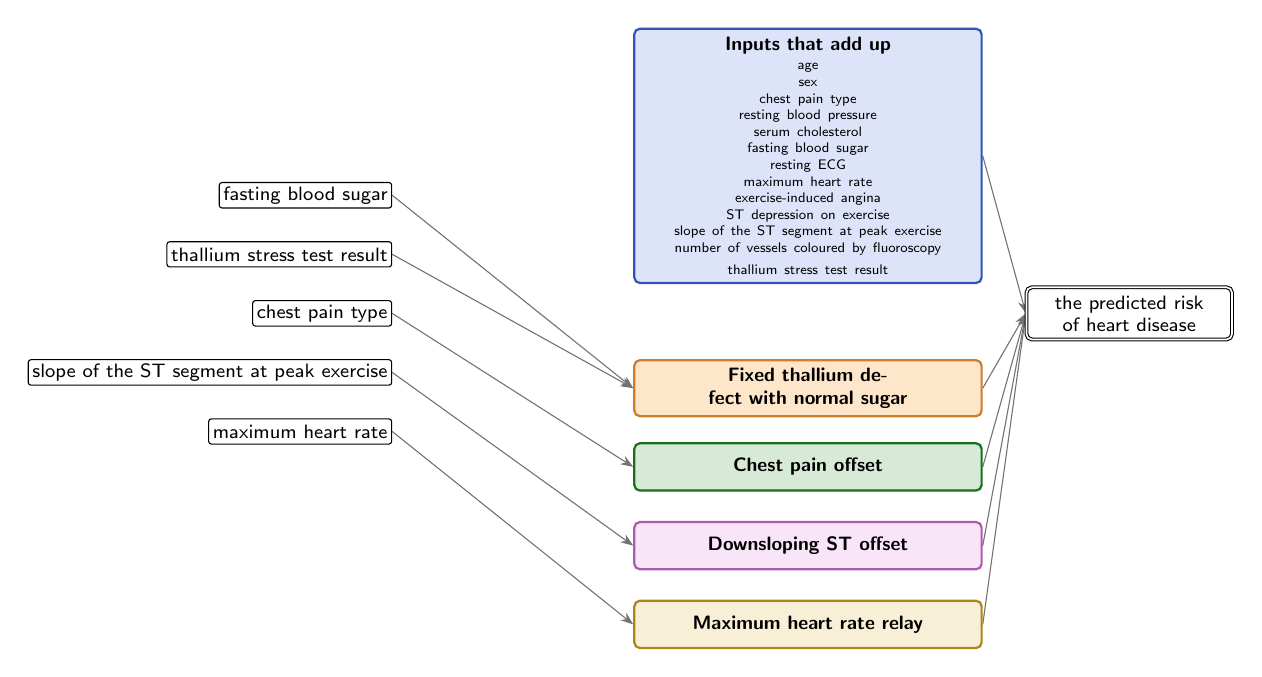
\begin{tikzpicture}[
  font=\sffamily\scriptsize, >={Stealth[length=1.6mm]},
  inp/.style={draw, rounded corners=1pt, fill=white, inner sep=1.5pt, minimum height=3.2mm, anchor=east},
  abox/.style={draw, thick, rounded corners=2pt, align=center, inner sep=3pt, minimum height=6mm, text width=42mm},
  outp/.style={draw, double, rounded corners=2pt, fill=white, align=center, inner sep=3pt, text width=24mm},
  agg/.style={draw=black!55},
]
\node[inp] (i0) at (0,1.5) {fasting blood sugar};
\node[inp] (i1) at (0,0.75) {thallium stress test result};
\node[inp] (i2) at (0,-0.0) {chest pain type};
\node[inp] (i3) at (0,-0.75) {slope of the ST segment at peak exercise};
\node[inp] (i4) at (0,-1.5) {maximum heart rate};
\node[abox, fill=RoyalBlue!18, draw=RoyalBlue!80!black] (b0) at (5.28,2.0) {\textbf{Inputs that add up}\\[1pt]{\tiny age\\ sex\\ chest pain type\\ resting blood pressure\\ serum cholesterol\\ fasting blood sugar\\ resting ECG\\ maximum heart rate\\ exercise-induced angina\\ ST depression on exercise\\ slope of the ST segment at peak exercise\\ number of vessels coloured by fluoroscopy\\ thallium stress test result}};
\node[abox, fill=BurntOrange!18, draw=BurntOrange!80!black] (b1) at (5.28,-0.95) {\textbf{Fixed thallium defect with normal sugar}};
\node[abox, fill=ForestGreen!18, draw=ForestGreen!80!black] (b2) at (5.28,-1.95) {\textbf{Chest pain offset}};
\node[abox, fill=Orchid!18, draw=Orchid!80!black] (b3) at (5.28,-2.95) {\textbf{Downsloping ST offset}};
\node[abox, fill=Goldenrod!18, draw=Goldenrod!80!black] (b4) at (5.28,-3.95) {\textbf{Maximum heart rate relay}};
\node[outp] (out) at (9.36,0) {the predicted risk of heart disease};
\begin{scope}[on background layer]
\draw[->, agg] (b0.east) -- (out.west);
\draw[->, agg, thin] (i0.east) -- (b1.west);
\draw[->, agg, thin] (i1.east) -- (b1.west);
\draw[->, agg] (b1.east) -- (out.west);
\draw[->, agg, thin] (i2.east) -- (b2.west);
\draw[->, agg] (b2.east) -- (out.west);
\draw[->, agg, thin] (i3.east) -- (b3.west);
\draw[->, agg] (b3.east) -- (out.west);
\draw[->, agg, thin] (i4.east) -- (b4.west);
\draw[->, agg] (b4.east) -- (out.west);
\end{scope}
\end{tikzpicture}}}%
\caption{The model at the level of the summary: one box per part.}
\label{fig:hearts4c1:summary}
\end{figure}
\paragraph{Inputs that add up.} \par\noindent\textit{Lowering the risk.}  These add up independently, and these lower the risk: being a woman takes a typical patient's predicted risk from about 24\% to about 1\%; through this sum alone, compared with no chest pain symptoms, typical angina lowers it to about 2\%, non-anginal chest pain to about 3\% and atypical angina to about 14\%, fasting blood sugar above 120 mg/dL lowers it to about 7\%, and a higher maximum heart rate lowers it steadily, from about 27\% at 118 to about 21\% at 175 beats per minute; chest pain type, fasting blood sugar and maximum heart rate also act through the parts below.\,{\scriptsize\textcolor{NavyBlue}{[C12, C13, C15, C22, C17, C24]}} \par\noindent\textit{Raising the risk.}  Each extra vessel coloured by fluoroscopy adds about the same, from about 24\% at 0 to about 98\% at 2 vessels, flattening out near the top because the predicted risk cannot go much higher; through this sum alone a flat rather than upsloping ST segment raises it to about 82\% and any thallium result other than a normal scan to about 48\%, and chest pain brought on by exercise raises it to about 36\% (the ST segment and the thallium scan also act through the parts below).\,{\scriptsize\textcolor{NavyBlue}{[C01, C02, C06, C21]}} Higher cholesterol (from about 14\% at 193 mg/dL to about 44\% at 308 mg/dL), more ST depression on exercise (from about 18\% at 0 mm to about 42\% at 2.8 mm), higher resting blood pressure (from about 14\% at 110 mm Hg to about 41\% at 155 mm Hg) and older age (from about 21\% at 42 to about 25\% at 66 years) raise it steadily.\,{\scriptsize\textcolor{NavyBlue}{[C04, C08, C05, C25]}} \par\noindent\textit{Rare results.}  Through this sum alone a downsloping ST segment raises it to about 39\% (the model has little data on this, n = 17), and an ST-T wave abnormality on the resting ECG raises it to about 38\% (the model has little data on this, n = 2).\,{\scriptsize\textcolor{NavyBlue}{[C19, C20]}}
\paragraph{Fixed thallium defect with normal sugar.} This part reads fasting blood sugar and the thallium scan and acts on 10 of 242 training patients, nearly all of them with a fixed defect on the thallium scan, 5 of whom had heart disease; for the typical patient it acts on, the predicted risk is about 94\% without it and about 24\% with it (the model has little data on this, n = 10).\,{\scriptsize\textcolor{NavyBlue}{[C35]}} Through it, a fixed defect on the thallium scan lowers a typical patient's predicted risk from about 24\% to about 2\% if fasting blood sugar is 120 mg/dL or less, but the other way if it is above 120 mg/dL, from about 7\% to about 18\% (the model has little data on this, n = 15).\,{\scriptsize\textcolor{NavyBlue}{[C34]}} For the typical patient it acts on, fasting blood sugar above 120 mg/dL raises the risk through it from about 24\% to about 94\%.\,{\scriptsize\textcolor{NavyBlue}{[C32]}}
\paragraph{Chest pain offset.} This part reads only chest pain type and acts on the 134 of 242 training patients who have some chest pain symptom, 30 of whom had heart disease; for the typical patient it acts on, the predicted risk is about 2\% without it and about 1\% with it.\,{\scriptsize\textcolor{NavyBlue}{[C38]}} Through it, any chest pain type other than no chest pain symptoms lowers a typical patient's predicted risk from about 24\% to about 12\%.\,{\scriptsize\textcolor{NavyBlue}{[C37]}}
\paragraph{Downsloping ST offset.} This part reads only the slope of the ST segment and acts on the 17 of 242 training patients with a downsloping ST segment, 8 of whom had heart disease; for the typical patient it acts on, the predicted risk is about 66\% without it and about 73\% with it (the model has little data on this, n = 17).\,{\scriptsize\textcolor{NavyBlue}{[C41]}} Through it, a downsloping ST segment raises a typical patient's predicted risk from about 24\% to about 29\% (the model has little data on this, n = 17).\,{\scriptsize\textcolor{NavyBlue}{[C40]}}
\paragraph{Maximum heart rate relay.} This part reads only maximum heart rate and acts on 190 of 242 training patients, 71 of whom had heart disease; for the typical patient it acts on, the predicted risk is about 21\% without it and about 20\% with it.\,{\scriptsize\textcolor{NavyBlue}{[C45]}} Through it, a higher maximum heart rate changes nothing until about 131 beats per minute, then lowers the predicted risk steadily, for a typical patient from about 24\% at 118 to about 23\% at 175 beats per minute.\,{\scriptsize\textcolor{NavyBlue}{[C43, C44]}}
\paragraph{The whole network.} Figure~\ref{fig:hearts4c1:overview} (next page, landscape) draws every unit and connection of the explained model, nested by part: shaded clusters are the parts of the model and darker boxes the parts inside them; circles are hidden units (h1, h2, \ldots); each cluster's rectangle is its output, and a dashed `sum' stands for an addition the next unit does (drawn, not a unit of the model); the hexagon is the model's output. An input used by several parts is drawn under each of them (same label, dotted outline, the first copy marked with the number of copies): it is the same input, repeated for readability. Not used by the model (input columns with no connection): atypical angina, normal ECG, LVH on ECG, no exercise pain, thallium code 4, reversible defect.
\begin{landscape}
\begin{figure}[p]\centering
\resizebox{\linewidth}{!}{%
\definecolor{netup}{HTML}{D95F02}\definecolor{netdown}{HTML}{1B9E77}\definecolor{netmixed}{HTML}{7F7F7F}%
\begin{tikzpicture}[
  font=\sffamily\scriptsize, >={Stealth[length=1.4mm]},
  inp/.style={draw, circle, fill=white, minimum size=3.2mm, inner sep=0pt},
  hid/.style={draw, circle, fill=white, minimum size=5.2mm, inner sep=0.5pt, font=\sffamily\tiny},
  exitbox/.style={draw, thick, rectangle, fill=white, align=center, text width=17mm, minimum height=5mm, inner sep=1.5pt, font=\sffamily\tiny},
  sumbox/.style={draw, thick, dashed, rectangle, fill=white, align=center, text width=17mm, minimum height=5mm, inner sep=1.5pt, font=\sffamily\tiny},
  outp/.style={draw, thick, regular polygon, regular polygon sides=6, fill=white, minimum size=10mm, inner sep=0pt, font=\sffamily\tiny, align=center},
  stub/.style={draw, dashed, rounded corners=2pt, fill=white, align=center, inner sep=2pt, font=\sffamily\tiny, text width=15mm},
  inlab/.style={font=\sffamily\tiny, align=center, text width=15mm, inner sep=1pt, fill=white, fill opacity=0.8, text opacity=1},
  wpos/.style={draw=NavyBlue}, wneg/.style={draw=BrickRed}, wagg/.style={draw=black!45, line width=1.2pt},
  wmix/.style={draw=Plum},
]
\node[outp] (n0) at (18.28,3.45) {heart disease};
\node[exitbox] (n1754) at (24.28,1.9) {Chest pain offset $\downarrow$};
\node[exitbox] (n2065) at (17.14,1.9) {Fixed thallium defect with normal sugar $\downarrow$};
\node[exitbox] (n3504) at (29.62,1.9) {Downsloping ST offset $\uparrow$};
\node[exitbox] (n707) at (35.66,1.9) {Maximum heart rate relay $\downarrow$};
\node[sumbox] (nxxsumxx) at (5.85,1.9) {sum: Inputs that add up};
\node[inp, draw=netup, very thick] (ninxxagexxadditive) at (1.8,-1.05) {};
\path (ninxxagexxadditive.south) node[inlab, anchor=north] (labninxxagexxadditive) {age $\uparrow$};
\node[inp, draw=netdown, very thick] (ninxxsexx0xxadditive) at (4.5,0.0) {};
\path (ninxxsexx0xxadditive.south) node[inlab, anchor=north] (labninxxsexx0xxadditive) {female $\downarrow$};
\node[inp, draw=netup, very thick] (ninxxsexx1xxadditive) at (5.4,-1.05) {};
\path (ninxxsexx1xxadditive.south) node[inlab, anchor=north] (labninxxsexx1xxadditive) {male $\uparrow$};
\node[inp, draw=netdown, very thick] (ninxxcpx1xxadditive) at (9.9,0.0) {};
\path (ninxxcpx1xxadditive.south) node[inlab, anchor=north] (labninxxcpx1xxadditive) {typical angina $\downarrow$};
\node[inp, draw=netdown, very thick] (ninxxcpx3xxadditive) at (7.2,-1.05) {};
\path (ninxxcpx3xxadditive.south) node[inlab, anchor=north] (labninxxcpx3xxadditive) {non-anginal pain $\downarrow$};
\node[inp, draw=netup, very thick] (ninxxtrestbpsxxadditive) at (1.8,-3.15) {};
\path (ninxxtrestbpsxxadditive.south) node[inlab, anchor=north] (labninxxtrestbpsxxadditive) {blood pressure $\uparrow$};
\node[inp, draw=netup, very thick] (ninxxcholxxadditive) at (2.7,0.0) {};
\path (ninxxcholxxadditive.south) node[inlab, anchor=north] (labninxxcholxxadditive) {cholesterol $\uparrow$};
\node[inp, draw=netup, very thick] (ninxxrestecgx1xxadditive) at (0.9,-2.1) {};
\path (ninxxrestecgx1xxadditive.south) node[inlab, anchor=north] (labninxxrestecgx1xxadditive) {ST-T abnormal ECG $\uparrow$};
\node[inp, draw=netup, very thick] (ninxxexangx1xxadditive) at (3.6,-1.05) {};
\path (ninxxexangx1xxadditive.south) node[inlab, anchor=north] (labninxxexangx1xxadditive) {exercise pain $\uparrow$};
\node[inp, draw=netup, very thick] (ninxxoldpeakxxadditive) at (0.9,0.0) {};
\path (ninxxoldpeakxxadditive.south) node[inlab, anchor=north] (labninxxoldpeakxxadditive) {ST depression $\uparrow$};
\node[inp, draw=netdown, very thick] (ninxxslopex1xxadditive) at (9.9,-2.1) {};
\path (ninxxslopex1xxadditive.south) node[inlab, anchor=north] (labninxxslopex1xxadditive) {upsloping ST $\downarrow$};
\node[inp, draw=netup, very thick] (ninxxslopex2xxadditive) at (4.5,-2.1) {};
\path (ninxxslopex2xxadditive.south) node[inlab, anchor=north] (labninxxslopex2xxadditive) {flat ST $\uparrow$};
\node[inp, draw=netup, very thick] (ninxxcaxxadditive) at (10.8,-1.05) {};
\path (ninxxcaxxadditive.south) node[inlab, anchor=north] (labninxxcaxxadditive) {vessels $\uparrow$};
\node[inp, draw=netdown, very thick] (ninxxthalx3xxadditive) at (8.1,0.0) {};
\path (ninxxthalx3xxadditive.south) node[inlab, anchor=north] (labninxxthalx3xxadditive) {normal thallium $\downarrow$};
\node[inp, draw=netdown, very thick] (ninxxthalx6xxannx31) at (15.34,0.0) {};
\path (ninxxthalx6xxannx31.south) node[inlab, anchor=north] (labninxxthalx6xxannx31) {fixed defect $\downarrow$};
\node[inp, densely dotted, thick, draw=netup, very thick] (ninxxfbsx0xxadditive) at (8.1,-2.1) {};
\path (ninxxfbsx0xxadditive.south) node[inlab, anchor=north] (labninxxfbsx0xxadditive) {sugar 120 or less ($\times$2) $\uparrow$};
\node[inp, densely dotted, thick, draw=netdown, very thick] (ninxxfbsx0xxannx31) at (17.14,0.0) {};
\path (ninxxfbsx0xxannx31.south) node[inlab, anchor=north] (labninxxfbsx0xxannx31) {sugar 120 or less $\downarrow$};
\node[inp, densely dotted, thick, draw=netdown, very thick] (ninxxfbsx1xxadditive) at (9.0,-1.05) {};
\path (ninxxfbsx1xxadditive.south) node[inlab, anchor=north] (labninxxfbsx1xxadditive) {sugar above 120 ($\times$2) $\downarrow$};
\node[inp, densely dotted, thick, draw=netup, very thick] (ninxxfbsx1xxannx31) at (18.94,0.0) {};
\path (ninxxfbsx1xxannx31.south) node[inlab, anchor=north] (labninxxfbsx1xxannx31) {sugar above 120 $\uparrow$};
\node[inp, densely dotted, thick, draw=netdown, very thick] (ninxxthalachxxadditive) at (6.3,0.0) {};
\path (ninxxthalachxxadditive.south) node[inlab, anchor=north] (labninxxthalachxxadditive) {max heart rate ($\times$2) $\downarrow$};
\node[inp, densely dotted, thick, draw=netdown, very thick] (ninxxthalachxxannx34) at (35.66,0.0) {};
\path (ninxxthalachxxannx34.south) node[inlab, anchor=north] (labninxxthalachxxannx34) {max heart rate $\downarrow$};
\node[inp, densely dotted, thick, draw=netup, very thick] (ninxxslopex3xxadditive) at (2.7,-2.1) {};
\path (ninxxslopex3xxadditive.south) node[inlab, anchor=north] (labninxxslopex3xxadditive) {downsloping ST ($\times$2) $\uparrow$};
\node[inp, densely dotted, thick, draw=netup, very thick] (ninxxslopex3xxannx33) at (29.62,0.0) {};
\path (ninxxslopex3xxannx33.south) node[inlab, anchor=north] (labninxxslopex3xxannx33) {downsloping ST $\uparrow$};
\node[inp, densely dotted, thick, draw=netup, very thick] (ninxxcpx4xxadditive) at (6.3,-2.1) {};
\path (ninxxcpx4xxadditive.south) node[inlab, anchor=north] (labninxxcpx4xxadditive) {no chest pain ($\times$2) $\uparrow$};
\node[inp, densely dotted, thick, draw=netup, very thick] (ninxxcpx4xxannx32) at (24.28,0.0) {};
\path (ninxxcpx4xxannx32.south) node[inlab, anchor=north] (labninxxcpx4xxannx32) {no chest pain $\uparrow$};
\begin{scope}[on background layer]
\node[fit=(nxxsumxx) , inner sep=8pt, rounded corners=5pt, fill=RoyalBlue!10, draw=RoyalBlue!45] (clu0) {};
\node[fit=(n2065) , inner sep=8pt, rounded corners=5pt, fill=BurntOrange!10, draw=BurntOrange!45] (clu1) {};
\node[fit=(n1754) , inner sep=8pt, rounded corners=5pt, fill=ForestGreen!10, draw=ForestGreen!45] (clu2) {};
\node[fit=(n3504) , inner sep=8pt, rounded corners=5pt, fill=Orchid!10, draw=Orchid!45] (clu3) {};
\node[fit=(n707) , inner sep=8pt, rounded corners=5pt, fill=Goldenrod!10, draw=Goldenrod!45] (clu4) {};
\draw[->, wpos, line width=0.28pt] (ninxxagexxadditive) -- (nxxsumxx);
\draw[->, wneg, line width=0.45pt] (ninxxsexx0xxadditive) -- (nxxsumxx);
\draw[->, wpos, line width=0.56pt] (ninxxsexx1xxadditive) -- (nxxsumxx);
\draw[->, wneg, line width=0.49pt] (ninxxcpx1xxadditive) -- (nxxsumxx);
\draw[->, wneg, line width=0.51pt] (ninxxcpx3xxadditive) -- (nxxsumxx);
\draw[->, wpos, line width=0.46pt] (ninxxtrestbpsxxadditive) -- (nxxsumxx);
\draw[->, wpos, line width=0.48pt] (ninxxcholxxadditive) -- (nxxsumxx);
\draw[->, wpos, line width=0.27pt] (ninxxrestecgx1xxadditive) -- (nxxsumxx);
\draw[->, wpos, line width=0.35pt] (ninxxexangx1xxadditive) -- (nxxsumxx);
\draw[->, wpos, line width=0.42pt] (ninxxoldpeakxxadditive) -- (nxxsumxx);
\draw[->, wneg, line width=0.33pt] (ninxxslopex1xxadditive) -- (nxxsumxx);
\draw[->, wpos, line width=0.64pt] (ninxxslopex2xxadditive) -- (nxxsumxx);
\draw[->, wpos, line width=1.04pt] (ninxxcaxxadditive) -- (nxxsumxx);
\draw[->, wneg, line width=0.44pt] (ninxxthalx3xxadditive) -- (nxxsumxx);
\draw[->, wneg, line width=0.27pt] (n707) -- (n0);
\draw[->, wneg, line width=0.56pt] (n1754) -- (n0);
\draw[->, wneg, line width=0.63pt] (n2065) -- (n0);
\draw[->, wpos, line width=0.29pt] (n3504) -- (n0);
\draw[->, wpos, line width=0.56pt] (ninxxthalx6xxannx31) -- (n2065);
\draw[->, wneg, line width=0.28pt] (ninxxfbsx0xxadditive) -- (nxxsumxx);
\draw[->, wpos, line width=0.80pt] (ninxxfbsx0xxannx31) -- (n2065);
\draw[->, wneg, line width=0.45pt] (ninxxfbsx1xxadditive) -- (nxxsumxx);
\draw[->, wneg, line width=0.49pt] (ninxxfbsx1xxannx31) -- (n2065);
\draw[->, wneg, line width=0.29pt] (ninxxthalachxxadditive) -- (nxxsumxx);
\draw[->, wpos, line width=0.59pt] (ninxxthalachxxannx34) -- (n707);
\draw[->, wpos, line width=0.27pt] (ninxxslopex3xxadditive) -- (nxxsumxx);
\draw[->, wpos, line width=0.60pt] (ninxxslopex3xxannx33) -- (n3504);
\draw[->, wpos, line width=0.36pt] (ninxxcpx4xxadditive) -- (nxxsumxx);
\draw[->, wneg, line width=0.63pt] (ninxxcpx4xxannx32) -- (n1754);
\draw[->, wagg] (nxxsumxx) -- (n0);
\end{scope}
\node[font=\sffamily\scriptsize\bfseries, text=RoyalBlue!55!black, anchor=south west, inner sep=1pt, fill=white, fill opacity=0.85, text opacity=1] at (clu0.north west) {Inputs that add up};
\node[font=\sffamily\scriptsize\bfseries, text=BurntOrange!55!black, anchor=south west, inner sep=1pt, fill=white, fill opacity=0.85, text opacity=1] at (clu1.north west) {Fixed thallium defect with normal sugar};
\node[font=\sffamily\scriptsize\bfseries, text=ForestGreen!55!black, anchor=south west, inner sep=1pt, fill=white, fill opacity=0.85, text opacity=1] at (clu2.north west) {Chest pain offset};
\node[font=\sffamily\scriptsize\bfseries, text=Orchid!55!black, anchor=south west, inner sep=1pt, fill=white, fill opacity=0.85, text opacity=1] at (clu3.north west) {Downsloping ST offset};
\node[font=\sffamily\scriptsize\bfseries, text=Goldenrod!55!black, anchor=south west, inner sep=1pt, fill=white, fill opacity=0.85, text opacity=1] at (clu4.north west) {Maximum heart rate relay};
\end{tikzpicture}}%
\caption{Every unit and connection of the explained model, nested by part. Blue: positive weight (raises the score); red: negative weight (lowers it); thicker: larger weight. Orange outline and up arrow: raises the final prediction; teal and down arrow: lowers it; grey and double arrow: depends.}
\label{fig:hearts4c1:overview}
\end{figure}
\end{landscape}
\paragraph{Worth checking against what is known.} Worth checking: going from 0 to 2 vessels coloured moves a typical patient's predicted risk from about 24\% to about 98\%.\,{\scriptsize\textcolor{NavyBlue}{[C01]}} Worth checking: patients with typical angina get the lowest predicted risk of all chest pain types, below patients with no chest pain symptoms.\,{\scriptsize\textcolor{NavyBlue}{[C10, C11, C16]}} Worth checking: the model treats fasting blood sugar above 120 mg/dL as lowering the risk of heart disease (for a typical patient from about 24\% to about 7\%).\,{\scriptsize\textcolor{NavyBlue}{[C18]}} Worth checking: through one part, the model treats a fixed defect on the thallium scan as lowering the risk for patients with normal fasting blood sugar (for a typical patient from about 24\% to about 2\%), from only 15 training patients.\,{\scriptsize\textcolor{NavyBlue}{[C34]}}
\subsection{The model, read from the top down}
\noindent{\small Each part of the explanation in turn, from the whole model down to the smallest parts: what it does for the prediction (hypothesis), what was checked (evidence), a diagram one level down, and where to read on. The technical record of each part is in ``Technical detail'' at the end.\par}
\subsubsection{The whole model}\label{rd:ann35}
\noindent{\small Figure~\ref{fig:hearts4c1:parts-ann35} shows what feeds this part; Figure~\ref{fig:hearts4c1:units-ann35} its units and every connection into them (dashed boxes: connections from or to other parts, drawn in their own sections).\par}
\begin{figure}[H]\centering
\resizebox{!}{\ifdim\height>0.5\textheight 0.5\textheight\else\height\fi}{%
\resizebox{\ifdim\width>\linewidth\linewidth\else\width\fi}{!}{%
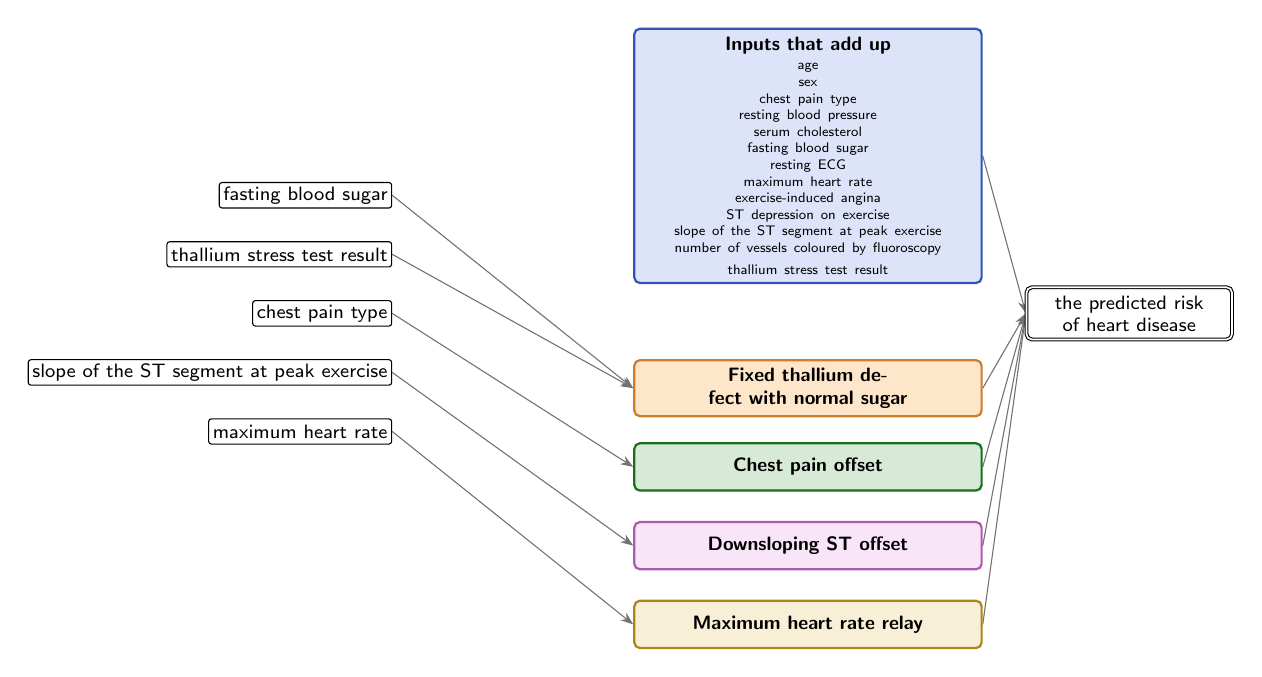
\begin{tikzpicture}[
  font=\sffamily\scriptsize, >={Stealth[length=1.6mm]},
  inp/.style={draw, rounded corners=1pt, fill=white, inner sep=1.5pt, minimum height=3.2mm, anchor=east},
  abox/.style={draw, thick, rounded corners=2pt, align=center, inner sep=3pt, minimum height=6mm, text width=42mm},
  outp/.style={draw, double, rounded corners=2pt, fill=white, align=center, inner sep=3pt, text width=24mm},
  agg/.style={draw=black!55},
]
\node[inp] (i0) at (0,1.5) {fasting blood sugar};
\node[inp] (i1) at (0,0.75) {thallium stress test result};
\node[inp] (i2) at (0,-0.0) {chest pain type};
\node[inp] (i3) at (0,-0.75) {slope of the ST segment at peak exercise};
\node[inp] (i4) at (0,-1.5) {maximum heart rate};
\node[abox, fill=RoyalBlue!18, draw=RoyalBlue!80!black] (b0) at (5.28,2.0) {\textbf{Inputs that add up}\\[1pt]{\tiny age\\ sex\\ chest pain type\\ resting blood pressure\\ serum cholesterol\\ fasting blood sugar\\ resting ECG\\ maximum heart rate\\ exercise-induced angina\\ ST depression on exercise\\ slope of the ST segment at peak exercise\\ number of vessels coloured by fluoroscopy\\ thallium stress test result}};
\node[abox, fill=BurntOrange!18, draw=BurntOrange!80!black] (b1) at (5.28,-0.95) {\textbf{Fixed thallium defect with normal sugar}};
\node[abox, fill=ForestGreen!18, draw=ForestGreen!80!black] (b2) at (5.28,-1.95) {\textbf{Chest pain offset}};
\node[abox, fill=Orchid!18, draw=Orchid!80!black] (b3) at (5.28,-2.95) {\textbf{Downsloping ST offset}};
\node[abox, fill=Goldenrod!18, draw=Goldenrod!80!black] (b4) at (5.28,-3.95) {\textbf{Maximum heart rate relay}};
\node[outp] (out) at (9.36,0) {the predicted risk of heart disease};
\begin{scope}[on background layer]
\draw[->, agg] (b0.east) -- (out.west);
\draw[->, agg, thin] (i0.east) -- (b1.west);
\draw[->, agg, thin] (i1.east) -- (b1.west);
\draw[->, agg] (b1.east) -- (out.west);
\draw[->, agg, thin] (i2.east) -- (b2.west);
\draw[->, agg] (b2.east) -- (out.west);
\draw[->, agg, thin] (i3.east) -- (b3.west);
\draw[->, agg] (b3.east) -- (out.west);
\draw[->, agg, thin] (i4.east) -- (b4.west);
\draw[->, agg] (b4.east) -- (out.west);
\end{scope}
\end{tikzpicture}}}%
\caption{The whole model: what feeds it, one level down.}
\label{fig:hearts4c1:parts-ann35}
\end{figure}
\begin{figure}[H]\centering
\resizebox{\ifdim\width>\linewidth\linewidth\else\width\fi}{!}{%
\definecolor{netup}{HTML}{D95F02}\definecolor{netdown}{HTML}{1B9E77}\definecolor{netmixed}{HTML}{7F7F7F}%
\begin{tikzpicture}[
  font=\sffamily\scriptsize, >={Stealth[length=1.4mm]},
  inp/.style={draw, circle, fill=white, minimum size=3.2mm, inner sep=0pt},
  hid/.style={draw, circle, fill=white, minimum size=5.2mm, inner sep=0.5pt, font=\sffamily\tiny},
  exitbox/.style={draw, thick, rectangle, fill=white, align=center, text width=17mm, minimum height=5mm, inner sep=1.5pt, font=\sffamily\tiny},
  sumbox/.style={draw, thick, dashed, rectangle, fill=white, align=center, text width=17mm, minimum height=5mm, inner sep=1.5pt, font=\sffamily\tiny},
  outp/.style={draw, thick, regular polygon, regular polygon sides=6, fill=white, minimum size=10mm, inner sep=0pt, font=\sffamily\tiny, align=center},
  stub/.style={draw, dashed, rounded corners=2pt, fill=white, align=center, inner sep=2pt, font=\sffamily\tiny, text width=15mm},
  inlab/.style={font=\sffamily\tiny, align=center, text width=15mm, inner sep=1pt, fill=white, fill opacity=0.8, text opacity=1},
  wpos/.style={draw=NavyBlue}, wneg/.style={draw=BrickRed}, wagg/.style={draw=black!45, line width=1.2pt},
  wmix/.style={draw=Plum},
]
\node[outp] (n0) at (10.22,3.45) {heart disease};
\node[inp, draw=netup, very thick] (ninxxage) at (1.8,-1.05) {};
\path (ninxxage.south) node[inlab, anchor=north] (labninxxage) {age $\uparrow$};
\node[sumbox] (nxxsumxx) at (5.85,1.9) {sum: Inputs that add up};
\node[inp, draw=netdown, very thick] (ninxxsexx0) at (4.5,0.0) {};
\path (ninxxsexx0.south) node[inlab, anchor=north] (labninxxsexx0) {female $\downarrow$};
\node[inp, draw=netup, very thick] (ninxxsexx1) at (5.4,-1.05) {};
\path (ninxxsexx1.south) node[inlab, anchor=north] (labninxxsexx1) {male $\uparrow$};
\node[inp, draw=netdown, very thick] (ninxxcpx1) at (9.9,0.0) {};
\path (ninxxcpx1.south) node[inlab, anchor=north] (labninxxcpx1) {typical angina $\downarrow$};
\node[inp, draw=netdown, very thick] (ninxxcpx3) at (7.2,-1.05) {};
\path (ninxxcpx3.south) node[inlab, anchor=north] (labninxxcpx3) {non-anginal pain $\downarrow$};
\node[inp, draw=netup, very thick] (ninxxtrestbps) at (1.8,-3.15) {};
\path (ninxxtrestbps.south) node[inlab, anchor=north] (labninxxtrestbps) {blood pressure $\uparrow$};
\node[inp, draw=netup, very thick] (ninxxchol) at (2.7,0.0) {};
\path (ninxxchol.south) node[inlab, anchor=north] (labninxxchol) {cholesterol $\uparrow$};
\node[inp, draw=netup, very thick] (ninxxrestecgx1) at (0.9,-2.1) {};
\path (ninxxrestecgx1.south) node[inlab, anchor=north] (labninxxrestecgx1) {ST-T abnormal ECG $\uparrow$};
\node[inp, draw=netup, very thick] (ninxxexangx1) at (3.6,-1.05) {};
\path (ninxxexangx1.south) node[inlab, anchor=north] (labninxxexangx1) {exercise pain $\uparrow$};
\node[inp, draw=netup, very thick] (ninxxoldpeak) at (0.9,0.0) {};
\path (ninxxoldpeak.south) node[inlab, anchor=north] (labninxxoldpeak) {ST depression $\uparrow$};
\node[inp, draw=netdown, very thick] (ninxxslopex1) at (9.9,-2.1) {};
\path (ninxxslopex1.south) node[inlab, anchor=north] (labninxxslopex1) {upsloping ST $\downarrow$};
\node[inp, draw=netup, very thick] (ninxxslopex2) at (4.5,-2.1) {};
\path (ninxxslopex2.south) node[inlab, anchor=north] (labninxxslopex2) {flat ST $\uparrow$};
\node[inp, draw=netup, very thick] (ninxxca) at (10.8,-1.05) {};
\path (ninxxca.south) node[inlab, anchor=north] (labninxxca) {vessels $\uparrow$};
\node[inp, draw=netdown, very thick] (ninxxthalx3) at (8.1,0.0) {};
\path (ninxxthalx3.south) node[inlab, anchor=north] (labninxxthalx3) {normal thallium $\downarrow$};
\node[stub] (nfromxxMaximumxheartxratexrelay) at (19.54,0.0) {from Maximum heart rate relay};
\node[stub] (nfromxxChestxpainxoffset) at (14.14,0.0) {from Chest pain offset};
\node[stub] (nfromxxFixedxthalliumxdefectxwithxnormalxsugar) at (17.74,0.0) {from Fixed thallium defect with normal sugar};
\node[stub] (nfromxxDownslopingxSTxoffset) at (15.94,0.0) {from Downsloping ST offset};
\node[inp, draw=netup, very thick] (ninxxfbsx0) at (8.1,-2.1) {};
\path (ninxxfbsx0.south) node[inlab, anchor=north] (labninxxfbsx0) {sugar 120 or less $\uparrow$};
\node[inp, draw=netdown, very thick] (ninxxfbsx1) at (9.0,-1.05) {};
\path (ninxxfbsx1.south) node[inlab, anchor=north] (labninxxfbsx1) {sugar above 120 $\downarrow$};
\node[inp, draw=netdown, very thick] (ninxxthalach) at (6.3,0.0) {};
\path (ninxxthalach.south) node[inlab, anchor=north] (labninxxthalach) {max heart rate $\downarrow$};
\node[inp, draw=netup, very thick] (ninxxslopex3) at (2.7,-2.1) {};
\path (ninxxslopex3.south) node[inlab, anchor=north] (labninxxslopex3) {downsloping ST $\uparrow$};
\node[inp, draw=netup, very thick] (ninxxcpx4) at (6.3,-2.1) {};
\path (ninxxcpx4.south) node[inlab, anchor=north] (labninxxcpx4) {no chest pain $\uparrow$};
\begin{scope}[on background layer]
\node[fit=(nxxsumxx) , inner sep=8pt, rounded corners=5pt, fill=RoyalBlue!10, draw=RoyalBlue!45] (clu0) {};
\draw[->, wpos, line width=0.28pt] (ninxxage) -- (nxxsumxx);
\draw[->, wneg, line width=0.45pt] (ninxxsexx0) -- (nxxsumxx);
\draw[->, wpos, line width=0.56pt] (ninxxsexx1) -- (nxxsumxx);
\draw[->, wneg, line width=0.49pt] (ninxxcpx1) -- (nxxsumxx);
\draw[->, wneg, line width=0.51pt] (ninxxcpx3) -- (nxxsumxx);
\draw[->, wpos, line width=0.46pt] (ninxxtrestbps) -- (nxxsumxx);
\draw[->, wpos, line width=0.48pt] (ninxxchol) -- (nxxsumxx);
\draw[->, wpos, line width=0.27pt] (ninxxrestecgx1) -- (nxxsumxx);
\draw[->, wpos, line width=0.35pt] (ninxxexangx1) -- (nxxsumxx);
\draw[->, wpos, line width=0.42pt] (ninxxoldpeak) -- (nxxsumxx);
\draw[->, wneg, line width=0.33pt] (ninxxslopex1) -- (nxxsumxx);
\draw[->, wpos, line width=0.64pt] (ninxxslopex2) -- (nxxsumxx);
\draw[->, wpos, line width=1.04pt] (ninxxca) -- (nxxsumxx);
\draw[->, wneg, line width=0.44pt] (ninxxthalx3) -- (nxxsumxx);
\draw[->, wneg, line width=0.27pt] (nfromxxMaximumxheartxratexrelay) -- (n0);
\draw[->, wneg, line width=0.56pt] (nfromxxChestxpainxoffset) -- (n0);
\draw[->, wneg, line width=0.63pt] (nfromxxFixedxthalliumxdefectxwithxnormalxsugar) -- (n0);
\draw[->, wpos, line width=0.29pt] (nfromxxDownslopingxSTxoffset) -- (n0);
\draw[->, wneg, line width=0.28pt] (ninxxfbsx0) -- (nxxsumxx);
\draw[->, wneg, line width=0.45pt] (ninxxfbsx1) -- (nxxsumxx);
\draw[->, wneg, line width=0.29pt] (ninxxthalach) -- (nxxsumxx);
\draw[->, wpos, line width=0.27pt] (ninxxslopex3) -- (nxxsumxx);
\draw[->, wpos, line width=0.36pt] (ninxxcpx4) -- (nxxsumxx);
\draw[->, wagg] (nxxsumxx) -- (n0);
\end{scope}
\node[font=\sffamily\scriptsize\bfseries, text=RoyalBlue!55!black, anchor=south west, inner sep=1pt, fill=white, fill opacity=0.85, text opacity=1] at (clu0.north west) {Inputs that add up};
\end{tikzpicture}}%
\caption{The whole model: its units and every connection into them. Blue: positive weight (raises the score); red: negative weight (lowers it); thicker: larger weight. Orange outline and up arrow: raises the final prediction; teal and down arrow: lowers it; grey and double arrow: depends.}
\label{fig:hearts4c1:units-ann35}
\end{figure}
\paragraph{Hypothesis.} The model adds up its inputs into one score: the vessels coloured (each extra vessel adding about the same), the ST segment, sex and chest pain type each move the predicted risk on their own, and four small parts add to that sum: one for a fixed thallium defect with normal fasting blood sugar, one for chest pain type, one for a downsloping ST segment and one for maximum heart rate.\,{\scriptsize\textcolor{NavyBlue}{[C31, C01, C02, C12, C10]}}
\paragraph{Evidence.} It is made up of the inputs that feed the score directly and four parts, the fixed thallium defect part, the chest pain offset, the downsloping ST offset and the maximum heart rate relay (each explained below); the score is their sum, which was checked on all 242 training patients.\,{\scriptsize\textcolor{NavyBlue}{[C31]}} Changing one input at a time across the whole model, compared with no chest pain symptoms, typical angina lowers a typical patient's predicted risk from about 24\% to about 1\%, non-anginal chest pain to about 1\% and atypical angina to about 7\%, against about 2\% for typical angina through the sum alone.\,{\scriptsize\textcolor{NavyBlue}{[C10, C11, C16, C13]}} Across the whole model, fasting blood sugar above 120 mg/dL lowers it from about 24\% to about 7\%, the same as through the sum alone.\,{\scriptsize\textcolor{NavyBlue}{[C18, C17]}} Across the whole model, a higher maximum heart rate lowers it slowly at first, then faster, from about 28\% at 118 to about 21\% at 175 beats per minute, against about 27\% to about 21\% through the sum alone, where it falls steadily.\,{\scriptsize\textcolor{NavyBlue}{[C23, C24]}} Across the whole model, a downsloping rather than upsloping ST segment raises it to about 47\% (the model has little data on this, n = 17), and a reversible defect on the thallium scan or a thallium result coded 4 raises it to about 48\%.\,{\scriptsize\textcolor{NavyBlue}{[C09, C07]}}
\par\noindent{\small Evidence plots: Figure~\ref{fig:hearts4c1:plot-ann35-0}.\par}
\begin{figure}[H]\centering
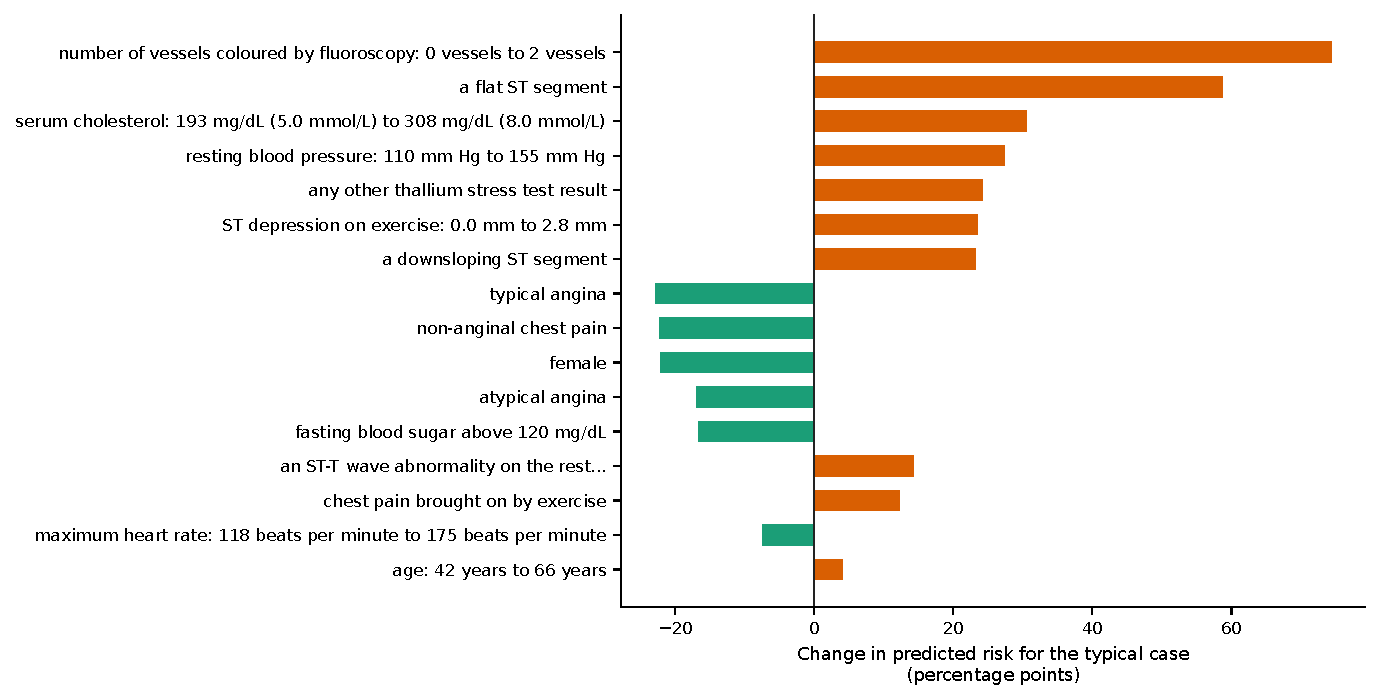
\includegraphics[width=\linewidth,height=0.88\textheight,keepaspectratio]{figures/heart-s4-c1/ann_35-effects.pdf}
\caption{The whole model: Each input's change in the predicted value for the typical case across the whole model, largest first (orange: raises it, teal: lowers it).}
\label{fig:hearts4c1:plot-ann35-0}
\end{figure}
\par\smallskip\noindent{\small \textbf{Dive deeper:} Fixed thallium defect with normal sugar (\ref{rd:ann31}); Chest pain offset (\ref{rd:ann32}); Downsloping ST offset (\ref{rd:ann33}); Maximum heart rate relay (\ref{rd:ann34}). Technical detail: \ref{tech:ann35}.\par}
\subsubsection{Fixed thallium defect with normal sugar}\label{rd:ann31}
\noindent{\footnotesize Part of: The whole model (\ref{rd:ann35}).\par}
\noindent{\small Figure~\ref{fig:hearts4c1:parts-ann31} shows what feeds this part; Figure~\ref{fig:hearts4c1:units-ann31} its units and every connection into them (dashed boxes: connections from or to other parts, drawn in their own sections).\par}
\begin{figure}[H]\centering
\resizebox{!}{\ifdim\height>0.5\textheight 0.5\textheight\else\height\fi}{%
\resizebox{\ifdim\width>\linewidth\linewidth\else\width\fi}{!}{%
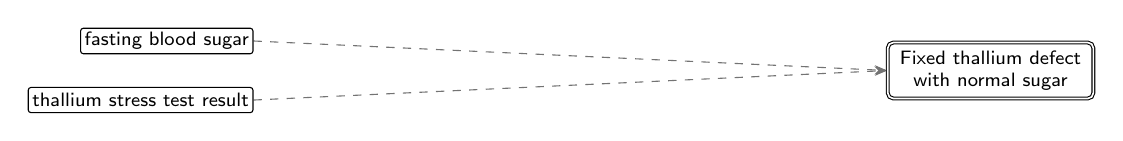
\begin{tikzpicture}[
  font=\sffamily\scriptsize, >={Stealth[length=1.6mm]},
  inp/.style={draw, rounded corners=1pt, fill=white, inner sep=1.5pt, minimum height=3.2mm, anchor=east},
  abox/.style={draw, thick, rounded corners=2pt, align=center, inner sep=3pt, minimum height=6mm, text width=42mm},
  outp/.style={draw, double, rounded corners=2pt, fill=white, align=center, inner sep=3pt, text width=24mm},
  agg/.style={draw=black!55},
]
\node[inp] (i0) at (0,0.375) {fasting blood sugar};
\node[inp] (i1) at (0,-0.375) {thallium stress test result};
\node[outp] (out) at (9.36,0) {Fixed thallium defect with normal sugar};
\begin{scope}[on background layer]
\draw[->, agg, thin, dashed] (i0.east) -- (out.west);
\draw[->, agg, thin, dashed] (i1.east) -- (out.west);
\end{scope}
\end{tikzpicture}}}%
\caption{Fixed thallium defect with normal sugar: what feeds it, one level down.}
\label{fig:hearts4c1:parts-ann31}
\end{figure}
\begin{figure}[H]\centering
\resizebox{\ifdim\width>\linewidth\linewidth\else\width\fi}{!}{%
\definecolor{netup}{HTML}{D95F02}\definecolor{netdown}{HTML}{1B9E77}\definecolor{netmixed}{HTML}{7F7F7F}%
\begin{tikzpicture}[
  font=\sffamily\scriptsize, >={Stealth[length=1.4mm]},
  inp/.style={draw, circle, fill=white, minimum size=3.2mm, inner sep=0pt},
  hid/.style={draw, circle, fill=white, minimum size=5.2mm, inner sep=0.5pt, font=\sffamily\tiny},
  exitbox/.style={draw, thick, rectangle, fill=white, align=center, text width=17mm, minimum height=5mm, inner sep=1.5pt, font=\sffamily\tiny},
  sumbox/.style={draw, thick, dashed, rectangle, fill=white, align=center, text width=17mm, minimum height=5mm, inner sep=1.5pt, font=\sffamily\tiny},
  outp/.style={draw, thick, regular polygon, regular polygon sides=6, fill=white, minimum size=10mm, inner sep=0pt, font=\sffamily\tiny, align=center},
  stub/.style={draw, dashed, rounded corners=2pt, fill=white, align=center, inner sep=2pt, font=\sffamily\tiny, text width=15mm},
  inlab/.style={font=\sffamily\tiny, align=center, text width=15mm, inner sep=1pt, fill=white, fill opacity=0.8, text opacity=1},
  wpos/.style={draw=NavyBlue}, wneg/.style={draw=BrickRed}, wagg/.style={draw=black!45, line width=1.2pt},
  wmix/.style={draw=Plum},
]
\node[exitbox] (n2065) at (3.9,1.9) {Fixed thallium defect with normal sugar $\downarrow$};
\node[inp, draw=netdown, very thick] (ninxxthalx6) at (2.1,0.0) {};
\path (ninxxthalx6.south) node[inlab, anchor=north] (labninxxthalx6) {fixed defect $\downarrow$};
\node[inp, draw=netdown, very thick] (ninxxfbsx0) at (3.9,0.0) {};
\path (ninxxfbsx0.south) node[inlab, anchor=north] (labninxxfbsx0) {sugar 120 or less $\downarrow$};
\node[inp, draw=netup, very thick] (ninxxfbsx1) at (5.7,0.0) {};
\path (ninxxfbsx1.south) node[inlab, anchor=north] (labninxxfbsx1) {sugar above 120 $\uparrow$};
\node[stub] (ntoxxthexmodelxoutput) at (3.9,3.45) {to the model output};
\begin{scope}[on background layer]
\node[fit=(n2065) , inner sep=8pt, rounded corners=5pt, fill=BurntOrange!10, draw=BurntOrange!45] (clu0) {};
\draw[->, wpos, line width=0.56pt] (ninxxthalx6) -- (n2065);
\draw[->, wpos, line width=0.80pt] (ninxxfbsx0) -- (n2065);
\draw[->, wneg, line width=0.49pt] (ninxxfbsx1) -- (n2065);
\draw[->, wneg, line width=0.63pt] (n2065) -- (ntoxxthexmodelxoutput);
\end{scope}
\node[font=\sffamily\scriptsize\bfseries, text=BurntOrange!55!black, anchor=south west, inner sep=1pt, fill=white, fill opacity=0.85, text opacity=1] at (clu0.north west) {Fixed thallium defect with normal sugar};
\end{tikzpicture}}%
\caption{Fixed thallium defect with normal sugar: its units and every connection into them. Blue: positive weight (raises the score); red: negative weight (lowers it); thicker: larger weight. Orange outline and up arrow: raises the final prediction; teal and down arrow: lowers it; grey and double arrow: depends.}
\label{fig:hearts4c1:units-ann31}
\end{figure}
\paragraph{Hypothesis.} This part lowers the predicted risk for patients with a fixed defect on the thallium scan when their fasting blood sugar is 120 mg/dL or less (the model has little data on this, n = 15).\,{\scriptsize\textcolor{NavyBlue}{[C34, C35]}}
\paragraph{Evidence.} It acts on 10 of 242 training patients, nearly all of them with a fixed defect on the thallium scan, 5 of whom had heart disease; for the typical patient it acts on, the predicted risk is about 94\% without it and about 24\% with it (the model has little data on this, n = 10).\,{\scriptsize\textcolor{NavyBlue}{[C35]}} Through it, a fixed defect on the thallium scan lowers a typical patient's predicted risk from about 24\% to below 1\% (the model has little data on this, n = 15).\,{\scriptsize\textcolor{NavyBlue}{[C33]}} Through it, a fixed defect lowers the risk from about 24\% to about 2\% if fasting blood sugar is 120 mg/dL or less, but raises it from about 7\% to about 18\% if it is above 120 mg/dL (the model has little data on this, n = 15).\,{\scriptsize\textcolor{NavyBlue}{[C34]}} For the typical patient it acts on, fasting blood sugar above 120 mg/dL raises the risk through it from about 24\% to about 94\%.\,{\scriptsize\textcolor{NavyBlue}{[C32]}} Its formula reproduces the part exactly on all 242 training patients.\,{\scriptsize\textcolor{NavyBlue}{[C36]}}
\par\noindent{\small Evidence plots: Figure~\ref{fig:hearts4c1:plot-ann31-0}, Figure~\ref{fig:hearts4c1:plot-ann31-1}, Figure~\ref{fig:hearts4c1:plot-ann31-2}.\par}
\par\noindent{\small Figure~\ref{fig:hearts4c1:plot-ann31-1} shows this part's own output, unit h3.\par}
\begin{figure}[H]\centering
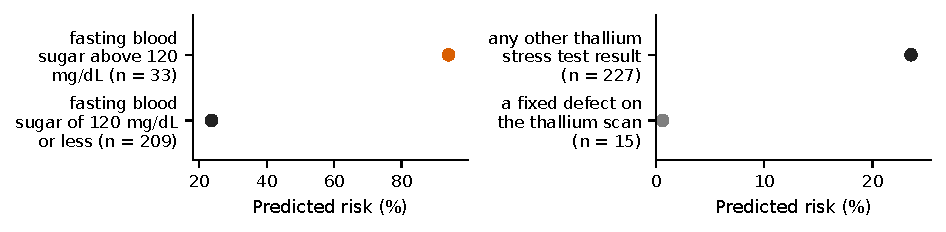
\includegraphics[width=\linewidth,height=0.88\textheight,keepaspectratio]{figures/heart-s4-c1/ann_31-categories-small.pdf}
\caption{Fixed thallium defect with normal sugar: The predicted value for the typical case at each level, through this part (n = training patients; grey: fewer than 20).}
\label{fig:hearts4c1:plot-ann31-0}
\end{figure}
\begin{figure}[H]\centering
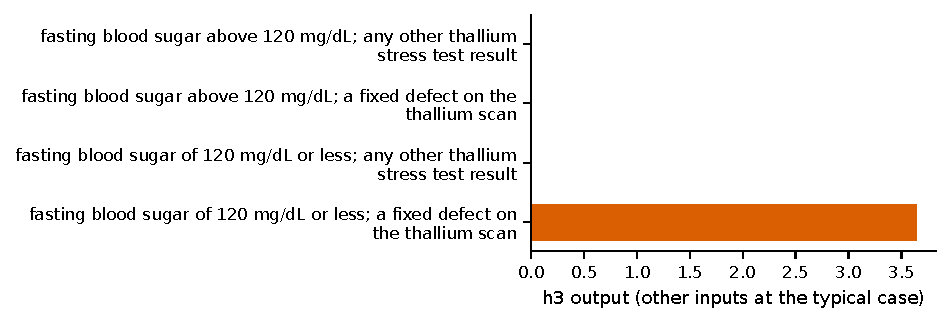
\includegraphics[width=\linewidth,height=0.88\textheight,keepaspectratio]{figures/heart-s4-c1/ann_31-partial-2065.pdf}
\caption{Fixed thallium defect with normal sugar: This part's own output, unit h3 (the output of 'Fixed thallium defect with normal sugar'), on its own scale (its activation), with every other input at the typical case; it is active for 10 of 242. Its output for each combination of the levels it reads.}
\label{fig:hearts4c1:plot-ann31-1}
\end{figure}
\begin{figure}[H]\centering
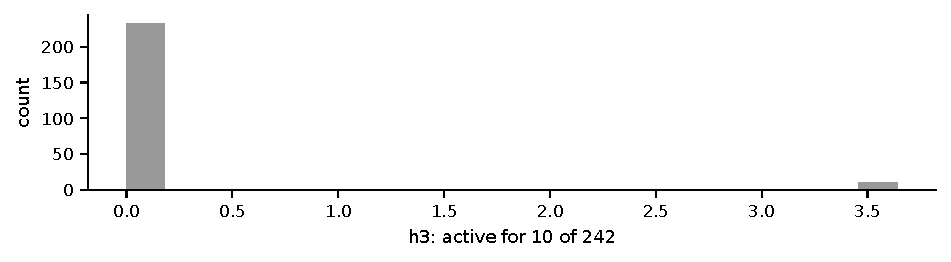
\includegraphics[width=\linewidth,height=0.88\textheight,keepaspectratio]{figures/heart-s4-c1/ann_31-units.pdf}
\caption{Fixed thallium defect with normal sugar: This part's hidden units: each unit's output against its main numeric input (top) and how often it is active (bottom).}
\label{fig:hearts4c1:plot-ann31-2}
\end{figure}
\par\smallskip\noindent{\small Technical detail: \ref{tech:ann31}.\par}
\subsubsection{Chest pain offset}\label{rd:ann32}
\noindent{\footnotesize Part of: The whole model (\ref{rd:ann35}).\par}
\noindent{\small Figure~\ref{fig:hearts4c1:parts-ann32} shows what feeds this part; Figure~\ref{fig:hearts4c1:units-ann32} its units and every connection into them (dashed boxes: connections from or to other parts, drawn in their own sections).\par}
\begin{figure}[H]\centering
\resizebox{!}{\ifdim\height>0.5\textheight 0.5\textheight\else\height\fi}{%
\resizebox{\ifdim\width>\linewidth\linewidth\else\width\fi}{!}{%
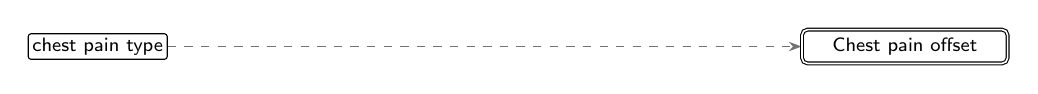
\begin{tikzpicture}[
  font=\sffamily\scriptsize, >={Stealth[length=1.6mm]},
  inp/.style={draw, rounded corners=1pt, fill=white, inner sep=1.5pt, minimum height=3.2mm, anchor=east},
  abox/.style={draw, thick, rounded corners=2pt, align=center, inner sep=3pt, minimum height=6mm, text width=42mm},
  outp/.style={draw, double, rounded corners=2pt, fill=white, align=center, inner sep=3pt, text width=24mm},
  agg/.style={draw=black!55},
]
\node[inp] (i0) at (0,-0.0) {chest pain type};
\node[outp] (out) at (9.36,0) {Chest pain offset};
\begin{scope}[on background layer]
\draw[->, agg, thin, dashed] (i0.east) -- (out.west);
\end{scope}
\end{tikzpicture}}}%
\caption{Chest pain offset: what feeds it, one level down.}
\label{fig:hearts4c1:parts-ann32}
\end{figure}
\begin{figure}[H]\centering
\resizebox{\ifdim\width>\linewidth\linewidth\else\width\fi}{!}{%
\definecolor{netup}{HTML}{D95F02}\definecolor{netdown}{HTML}{1B9E77}\definecolor{netmixed}{HTML}{7F7F7F}%
\begin{tikzpicture}[
  font=\sffamily\scriptsize, >={Stealth[length=1.4mm]},
  inp/.style={draw, circle, fill=white, minimum size=3.2mm, inner sep=0pt},
  hid/.style={draw, circle, fill=white, minimum size=5.2mm, inner sep=0.5pt, font=\sffamily\tiny},
  exitbox/.style={draw, thick, rectangle, fill=white, align=center, text width=17mm, minimum height=5mm, inner sep=1.5pt, font=\sffamily\tiny},
  sumbox/.style={draw, thick, dashed, rectangle, fill=white, align=center, text width=17mm, minimum height=5mm, inner sep=1.5pt, font=\sffamily\tiny},
  outp/.style={draw, thick, regular polygon, regular polygon sides=6, fill=white, minimum size=10mm, inner sep=0pt, font=\sffamily\tiny, align=center},
  stub/.style={draw, dashed, rounded corners=2pt, fill=white, align=center, inner sep=2pt, font=\sffamily\tiny, text width=15mm},
  inlab/.style={font=\sffamily\tiny, align=center, text width=15mm, inner sep=1pt, fill=white, fill opacity=0.8, text opacity=1},
  wpos/.style={draw=NavyBlue}, wneg/.style={draw=BrickRed}, wagg/.style={draw=black!45, line width=1.2pt},
  wmix/.style={draw=Plum},
]
\node[exitbox] (n1754) at (1.7,1.9) {Chest pain offset $\downarrow$};
\node[inp, draw=netup, very thick] (ninxxcpx4) at (1.7,0.0) {};
\path (ninxxcpx4.south) node[inlab, anchor=north] (labninxxcpx4) {no chest pain $\uparrow$};
\node[stub] (ntoxxthexmodelxoutput) at (1.7,3.45) {to the model output};
\begin{scope}[on background layer]
\node[fit=(n1754) , inner sep=8pt, rounded corners=5pt, fill=ForestGreen!10, draw=ForestGreen!45] (clu0) {};
\draw[->, wneg, line width=0.63pt] (ninxxcpx4) -- (n1754);
\draw[->, wneg, line width=0.56pt] (n1754) -- (ntoxxthexmodelxoutput);
\end{scope}
\node[font=\sffamily\scriptsize\bfseries, text=ForestGreen!55!black, anchor=south west, inner sep=1pt, fill=white, fill opacity=0.85, text opacity=1] at (clu0.north west) {Chest pain offset};
\end{tikzpicture}}%
\caption{Chest pain offset: its units and every connection into them. Blue: positive weight (raises the score); red: negative weight (lowers it); thicker: larger weight. Orange outline and up arrow: raises the final prediction; teal and down arrow: lowers it; grey and double arrow: depends.}
\label{fig:hearts4c1:units-ann32}
\end{figure}
\paragraph{Hypothesis.} This part lowers the predicted risk for patients with any chest pain symptom, compared with patients who have none.\,{\scriptsize\textcolor{NavyBlue}{[C37]}}
\paragraph{Evidence.} It acts on the 134 of 242 training patients who have some chest pain symptom, 30 of whom had heart disease; for the typical patient it acts on, the predicted risk is about 2\% without it and about 1\% with it.\,{\scriptsize\textcolor{NavyBlue}{[C38]}} Through it, any chest pain type other than no chest pain symptoms takes a typical patient's predicted risk from about 24\% to about 12\%.\,{\scriptsize\textcolor{NavyBlue}{[C37]}} Its formula reproduces the part exactly on all 242 training patients.\,{\scriptsize\textcolor{NavyBlue}{[C39]}}
\par\noindent{\small Evidence plots: Figure~\ref{fig:hearts4c1:plot-ann32-0}, Figure~\ref{fig:hearts4c1:plot-ann32-1}.\par}
\begin{figure}[H]\centering
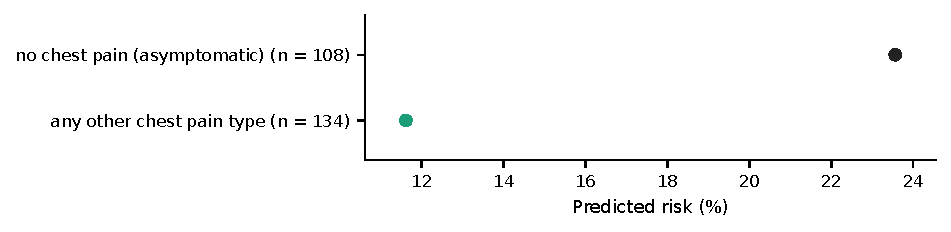
\includegraphics[width=\linewidth,height=0.88\textheight,keepaspectratio]{figures/heart-s4-c1/ann_32-categories-small.pdf}
\caption{Chest pain offset: The predicted value for the typical case at each level, through this part (n = training patients; grey: fewer than 20).}
\label{fig:hearts4c1:plot-ann32-0}
\end{figure}
\begin{figure}[H]\centering
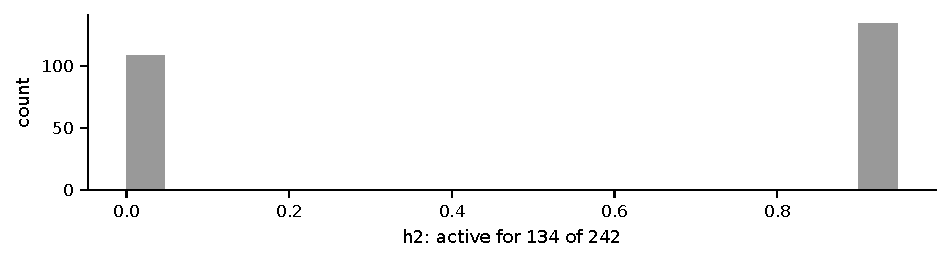
\includegraphics[width=\linewidth,height=0.88\textheight,keepaspectratio]{figures/heart-s4-c1/ann_32-units.pdf}
\caption{Chest pain offset: This part's hidden units: each unit's output against its main numeric input (top) and how often it is active (bottom).}
\label{fig:hearts4c1:plot-ann32-1}
\end{figure}
\par\smallskip\noindent{\small Technical detail: \ref{tech:ann32}.\par}
\subsubsection{Downsloping ST offset}\label{rd:ann33}
\noindent{\footnotesize Part of: The whole model (\ref{rd:ann35}).\par}
\noindent{\small Figure~\ref{fig:hearts4c1:parts-ann33} shows what feeds this part; Figure~\ref{fig:hearts4c1:units-ann33} its units and every connection into them (dashed boxes: connections from or to other parts, drawn in their own sections).\par}
\begin{figure}[H]\centering
\resizebox{!}{\ifdim\height>0.5\textheight 0.5\textheight\else\height\fi}{%
\resizebox{\ifdim\width>\linewidth\linewidth\else\width\fi}{!}{%
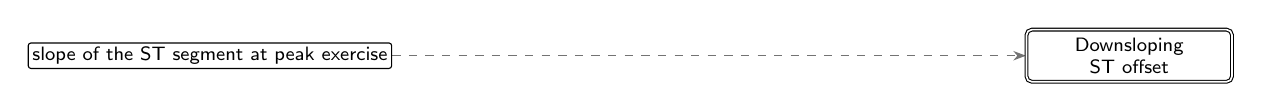
\begin{tikzpicture}[
  font=\sffamily\scriptsize, >={Stealth[length=1.6mm]},
  inp/.style={draw, rounded corners=1pt, fill=white, inner sep=1.5pt, minimum height=3.2mm, anchor=east},
  abox/.style={draw, thick, rounded corners=2pt, align=center, inner sep=3pt, minimum height=6mm, text width=42mm},
  outp/.style={draw, double, rounded corners=2pt, fill=white, align=center, inner sep=3pt, text width=24mm},
  agg/.style={draw=black!55},
]
\node[inp] (i0) at (0,-0.0) {slope of the ST segment at peak exercise};
\node[outp] (out) at (9.36,0) {Downsloping ST offset};
\begin{scope}[on background layer]
\draw[->, agg, thin, dashed] (i0.east) -- (out.west);
\end{scope}
\end{tikzpicture}}}%
\caption{Downsloping ST offset: what feeds it, one level down.}
\label{fig:hearts4c1:parts-ann33}
\end{figure}
\begin{figure}[H]\centering
\resizebox{\ifdim\width>\linewidth\linewidth\else\width\fi}{!}{%
\definecolor{netup}{HTML}{D95F02}\definecolor{netdown}{HTML}{1B9E77}\definecolor{netmixed}{HTML}{7F7F7F}%
\begin{tikzpicture}[
  font=\sffamily\scriptsize, >={Stealth[length=1.4mm]},
  inp/.style={draw, circle, fill=white, minimum size=3.2mm, inner sep=0pt},
  hid/.style={draw, circle, fill=white, minimum size=5.2mm, inner sep=0.5pt, font=\sffamily\tiny},
  exitbox/.style={draw, thick, rectangle, fill=white, align=center, text width=17mm, minimum height=5mm, inner sep=1.5pt, font=\sffamily\tiny},
  sumbox/.style={draw, thick, dashed, rectangle, fill=white, align=center, text width=17mm, minimum height=5mm, inner sep=1.5pt, font=\sffamily\tiny},
  outp/.style={draw, thick, regular polygon, regular polygon sides=6, fill=white, minimum size=10mm, inner sep=0pt, font=\sffamily\tiny, align=center},
  stub/.style={draw, dashed, rounded corners=2pt, fill=white, align=center, inner sep=2pt, font=\sffamily\tiny, text width=15mm},
  inlab/.style={font=\sffamily\tiny, align=center, text width=15mm, inner sep=1pt, fill=white, fill opacity=0.8, text opacity=1},
  wpos/.style={draw=NavyBlue}, wneg/.style={draw=BrickRed}, wagg/.style={draw=black!45, line width=1.2pt},
  wmix/.style={draw=Plum},
]
\node[exitbox] (n3504) at (2.1,1.9) {Downsloping ST offset $\uparrow$};
\node[inp, draw=netup, very thick] (ninxxslopex3) at (2.1,0.0) {};
\path (ninxxslopex3.south) node[inlab, anchor=north] (labninxxslopex3) {downsloping ST $\uparrow$};
\node[stub] (ntoxxthexmodelxoutput) at (2.1,3.45) {to the model output};
\begin{scope}[on background layer]
\node[fit=(n3504) , inner sep=8pt, rounded corners=5pt, fill=Orchid!10, draw=Orchid!45] (clu0) {};
\draw[->, wpos, line width=0.60pt] (ninxxslopex3) -- (n3504);
\draw[->, wpos, line width=0.29pt] (n3504) -- (ntoxxthexmodelxoutput);
\end{scope}
\node[font=\sffamily\scriptsize\bfseries, text=Orchid!55!black, anchor=south west, inner sep=1pt, fill=white, fill opacity=0.85, text opacity=1] at (clu0.north west) {Downsloping ST offset};
\end{tikzpicture}}%
\caption{Downsloping ST offset: its units and every connection into them. Blue: positive weight (raises the score); red: negative weight (lowers it); thicker: larger weight. Orange outline and up arrow: raises the final prediction; teal and down arrow: lowers it; grey and double arrow: depends.}
\label{fig:hearts4c1:units-ann33}
\end{figure}
\paragraph{Hypothesis.} This part raises the predicted risk a little for patients with a downsloping ST segment (the model has little data on this, n = 17).\,{\scriptsize\textcolor{NavyBlue}{[C40]}}
\paragraph{Evidence.} It acts on the 17 of 242 training patients with a downsloping ST segment, 8 of whom had heart disease; for the typical patient it acts on, the predicted risk is about 66\% without it and about 73\% with it (the model has little data on this, n = 17).\,{\scriptsize\textcolor{NavyBlue}{[C41]}} Through it, a downsloping ST segment takes a typical patient's predicted risk from about 24\% to about 29\% (the model has little data on this, n = 17).\,{\scriptsize\textcolor{NavyBlue}{[C40]}} Its formula reproduces the part exactly on all 242 training patients.\,{\scriptsize\textcolor{NavyBlue}{[C42]}}
\par\noindent{\small Evidence plots: Figure~\ref{fig:hearts4c1:plot-ann33-0}, Figure~\ref{fig:hearts4c1:plot-ann33-1}.\par}
\begin{figure}[H]\centering
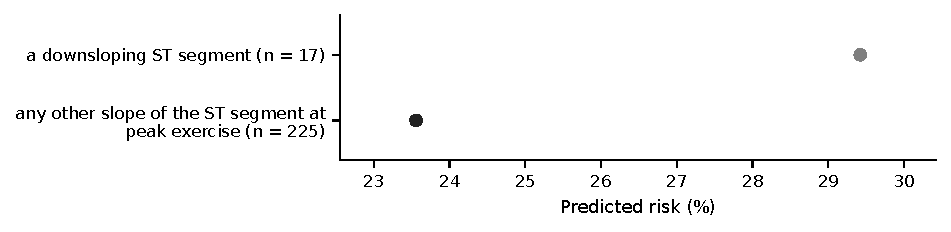
\includegraphics[width=\linewidth,height=0.88\textheight,keepaspectratio]{figures/heart-s4-c1/ann_33-categories-small.pdf}
\caption{Downsloping ST offset: The predicted value for the typical case at each level, through this part (n = training patients; grey: fewer than 20).}
\label{fig:hearts4c1:plot-ann33-0}
\end{figure}
\begin{figure}[H]\centering
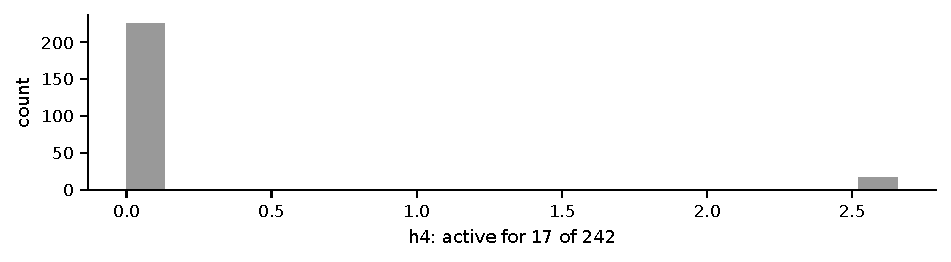
\includegraphics[width=\linewidth,height=0.88\textheight,keepaspectratio]{figures/heart-s4-c1/ann_33-units.pdf}
\caption{Downsloping ST offset: This part's hidden units: each unit's output against its main numeric input (top) and how often it is active (bottom).}
\label{fig:hearts4c1:plot-ann33-1}
\end{figure}
\par\smallskip\noindent{\small Technical detail: \ref{tech:ann33}.\par}
\subsubsection{Maximum heart rate relay}\label{rd:ann34}
\noindent{\footnotesize Part of: The whole model (\ref{rd:ann35}).\par}
\noindent{\small Figure~\ref{fig:hearts4c1:parts-ann34} shows what feeds this part; Figure~\ref{fig:hearts4c1:units-ann34} its units and every connection into them (dashed boxes: connections from or to other parts, drawn in their own sections).\par}
\begin{figure}[H]\centering
\resizebox{!}{\ifdim\height>0.5\textheight 0.5\textheight\else\height\fi}{%
\resizebox{\ifdim\width>\linewidth\linewidth\else\width\fi}{!}{%
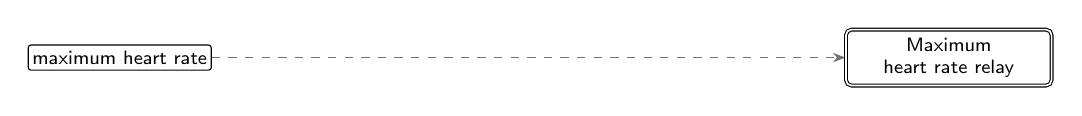
\begin{tikzpicture}[
  font=\sffamily\scriptsize, >={Stealth[length=1.6mm]},
  inp/.style={draw, rounded corners=1pt, fill=white, inner sep=1.5pt, minimum height=3.2mm, anchor=east},
  abox/.style={draw, thick, rounded corners=2pt, align=center, inner sep=3pt, minimum height=6mm, text width=42mm},
  outp/.style={draw, double, rounded corners=2pt, fill=white, align=center, inner sep=3pt, text width=24mm},
  agg/.style={draw=black!55},
]
\node[inp] (i0) at (0,-0.0) {maximum heart rate};
\node[outp] (out) at (9.36,0) {Maximum heart rate relay};
\begin{scope}[on background layer]
\draw[->, agg, thin, dashed] (i0.east) -- (out.west);
\end{scope}
\end{tikzpicture}}}%
\caption{Maximum heart rate relay: what feeds it, one level down.}
\label{fig:hearts4c1:parts-ann34}
\end{figure}
\begin{figure}[H]\centering
\resizebox{\ifdim\width>\linewidth\linewidth\else\width\fi}{!}{%
\definecolor{netup}{HTML}{D95F02}\definecolor{netdown}{HTML}{1B9E77}\definecolor{netmixed}{HTML}{7F7F7F}%
\begin{tikzpicture}[
  font=\sffamily\scriptsize, >={Stealth[length=1.4mm]},
  inp/.style={draw, circle, fill=white, minimum size=3.2mm, inner sep=0pt},
  hid/.style={draw, circle, fill=white, minimum size=5.2mm, inner sep=0.5pt, font=\sffamily\tiny},
  exitbox/.style={draw, thick, rectangle, fill=white, align=center, text width=17mm, minimum height=5mm, inner sep=1.5pt, font=\sffamily\tiny},
  sumbox/.style={draw, thick, dashed, rectangle, fill=white, align=center, text width=17mm, minimum height=5mm, inner sep=1.5pt, font=\sffamily\tiny},
  outp/.style={draw, thick, regular polygon, regular polygon sides=6, fill=white, minimum size=10mm, inner sep=0pt, font=\sffamily\tiny, align=center},
  stub/.style={draw, dashed, rounded corners=2pt, fill=white, align=center, inner sep=2pt, font=\sffamily\tiny, text width=15mm},
  inlab/.style={font=\sffamily\tiny, align=center, text width=15mm, inner sep=1pt, fill=white, fill opacity=0.8, text opacity=1},
  wpos/.style={draw=NavyBlue}, wneg/.style={draw=BrickRed}, wagg/.style={draw=black!45, line width=1.2pt},
  wmix/.style={draw=Plum},
]
\node[exitbox] (n707) at (2.4,1.9) {Maximum heart rate relay $\downarrow$};
\node[inp, draw=netdown, very thick] (ninxxthalach) at (2.4,0.0) {};
\path (ninxxthalach.south) node[inlab, anchor=north] (labninxxthalach) {max heart rate $\downarrow$};
\node[stub] (ntoxxthexmodelxoutput) at (2.4,3.45) {to the model output};
\begin{scope}[on background layer]
\node[fit=(n707) , inner sep=8pt, rounded corners=5pt, fill=Goldenrod!10, draw=Goldenrod!45] (clu0) {};
\draw[->, wpos, line width=0.59pt] (ninxxthalach) -- (n707);
\draw[->, wneg, line width=0.27pt] (n707) -- (ntoxxthexmodelxoutput);
\end{scope}
\node[font=\sffamily\scriptsize\bfseries, text=Goldenrod!55!black, anchor=south west, inner sep=1pt, fill=white, fill opacity=0.85, text opacity=1] at (clu0.north west) {Maximum heart rate relay};
\end{tikzpicture}}%
\caption{Maximum heart rate relay: its units and every connection into them. Blue: positive weight (raises the score); red: negative weight (lowers it); thicker: larger weight. Orange outline and up arrow: raises the final prediction; teal and down arrow: lowers it; grey and double arrow: depends.}
\label{fig:hearts4c1:units-ann34}
\end{figure}
\paragraph{Hypothesis.} Through this part, a higher maximum heart rate changes nothing until about 131 beats per minute, then lowers the predicted risk steadily.\,{\scriptsize\textcolor{NavyBlue}{[C43, C44]}}
\paragraph{Evidence.} It acts on 190 of 242 training patients, 71 of whom had heart disease; for the typical patient it acts on, the predicted risk is about 21\% without it and about 20\% with it.\,{\scriptsize\textcolor{NavyBlue}{[C45]}} Through it, a higher maximum heart rate changes nothing until about 131 beats per minute, then lowers the risk steadily, for a typical patient from about 24\% at 118 to about 23\% at 175 beats per minute.\,{\scriptsize\textcolor{NavyBlue}{[C43, C44]}} Its formula reproduces the part exactly on all 242 training patients.\,{\scriptsize\textcolor{NavyBlue}{[C47]}}
\par\noindent{\small Evidence plots: Figure~\ref{fig:hearts4c1:plot-ann34-0}, Figure~\ref{fig:hearts4c1:plot-ann34-1}, Figure~\ref{fig:hearts4c1:plot-ann34-2}.\par}
\par\noindent{\small Figure~\ref{fig:hearts4c1:plot-ann34-1} shows this part's own output, unit h1: it switches on at about 131.1 beats per minute of maximum heart rate, and is zero below.\par}
\begin{figure}[H]\centering
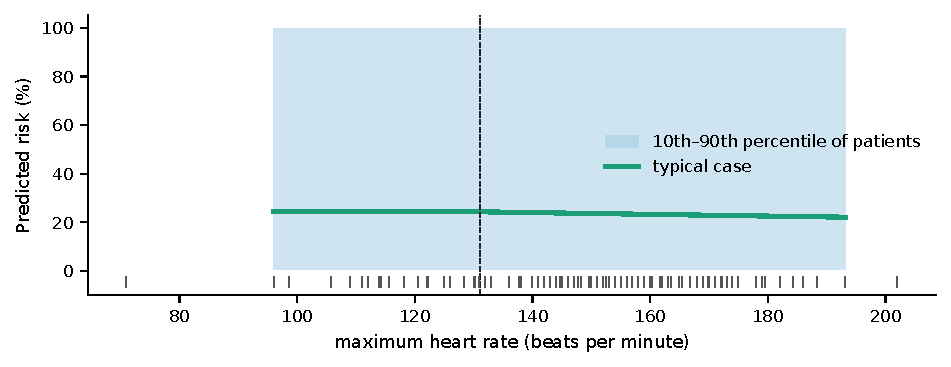
\includegraphics[width=\linewidth,height=0.88\textheight,keepaspectratio]{figures/heart-s4-c1/ann_34-response.pdf}
\caption{Maximum heart rate relay: Response curves through this part: the typical case (bold), the 10th to 90th percentile of individual patients (band), the fold or step point (dashed) with its spread across them (grey), and the observed values (ticks).}
\label{fig:hearts4c1:plot-ann34-0}
\end{figure}
\begin{figure}[H]\centering
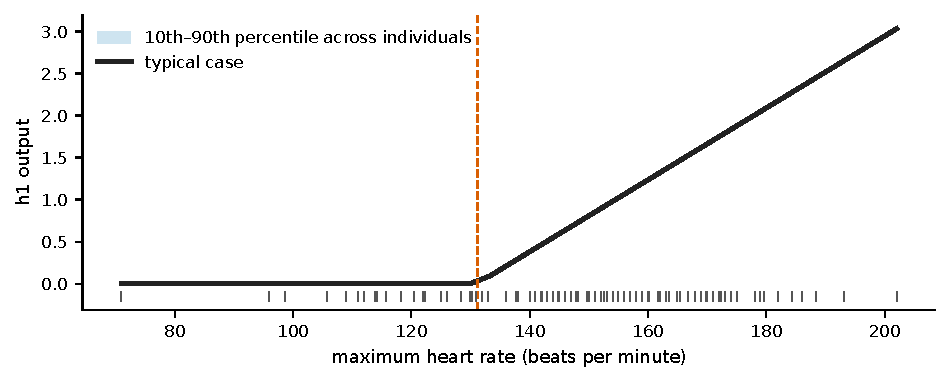
\includegraphics[width=\linewidth,height=0.88\textheight,keepaspectratio]{figures/heart-s4-c1/ann_34-partial-707.pdf}
\caption{Maximum heart rate relay: This part's own output, unit h1 (the output of 'Maximum heart rate relay'), on its own scale (its activation), with every other input at the typical case; it is active for 190 of 242. Bold: the typical case; band: 10th to 90th percentile across individuals; dashed: where it switches on; ticks: the data.}
\label{fig:hearts4c1:plot-ann34-1}
\end{figure}
\begin{figure}[H]\centering
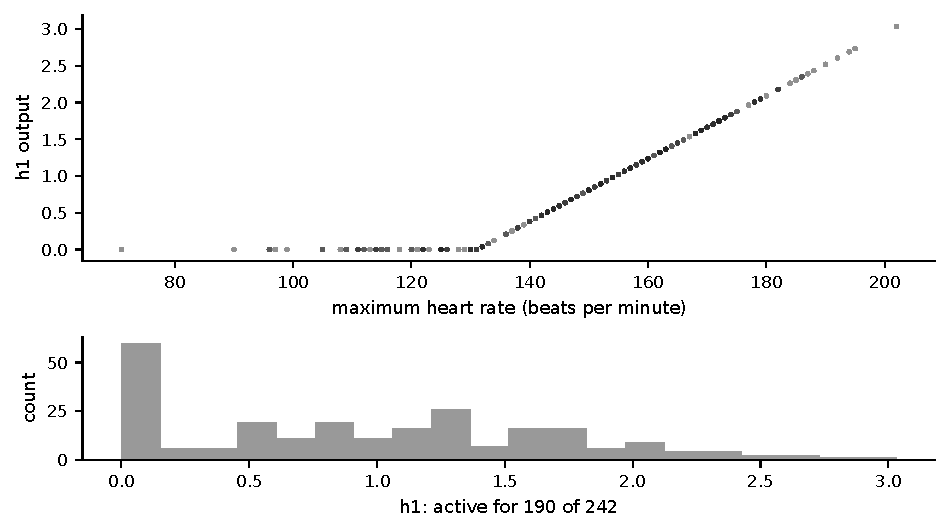
\includegraphics[width=\linewidth,height=0.88\textheight,keepaspectratio]{figures/heart-s4-c1/ann_34-units.pdf}
\caption{Maximum heart rate relay: This part's hidden units: each unit's output against its main numeric input (top) and how often it is active (bottom).}
\label{fig:hearts4c1:plot-ann34-2}
\end{figure}
\par\smallskip\noindent{\small Technical detail: \ref{tech:ann34}.\par}
\subsection{Not supported by the model}
\begin{itemize}\setlength\itemsep{0pt}\small
\item C14: direction claim about thallium stress test result in the whole model: not supported by the model (14\% of patients have the opposite sign (allowed: 10\%)).
\item C46: null claim about maximum heart rate reached during the exercise test in part ann\_\allowbreak{}34: not supported by the model (predictions move by up to 0.026).
\end{itemize}
\clearpage\section*{Technical detail: heart-s4-c1}
\addcontentsline{toc}{section}{Technical detail: heart-s4-c1}
\noindent{\small The record behind each part: the original hypothesis, the closed form, and every claim with its estimate (log-odds and odds ratio), range across patients, n and test check.\par}
\renewcommand{\thesubsection}{T.\arabic{subsection}}\setcounter{subsection}{0}
\subsection{The whole model}\label{tech:ann35}
\noindent{\footnotesize Annotation ann\_\allowbreak{}35 (heart\_\allowbreak{}disease\_\allowbreak{}logit). Reads: age, sex, chest pain type, resting blood pressure, serum cholesterol, fasting blood sugar, resting ECG, maximum heart rate reached during the exercise test, exercise-induced angina, ST depression during exercise (compared with rest), slope of the ST segment at peak exercise, number of major vessels coloured by fluoroscopy, thallium stress test result.\par}
\paragraph{Original hypothesis (unchanged).} Root: p = sigmoid(z), z = 0.466 + LINEAR CORE - 1.077*\allowbreak{}fixed\_\allowbreak{}defect\_\allowbreak{}normal\_\allowbreak{}sugar\_\allowbreak{}gate - 0.899*\allowbreak{}no\_\allowbreak{}asymptomatic\_\allowbreak{}pain\_\allowbreak{}indicator + 0.114*\allowbreak{}downsloping\_\allowbreak{}st\_\allowbreak{}indicator - 0.047*\allowbreak{}thalach\_\allowbreak{}floor\_\allowbreak{}relay. LINEAR CORE (19 direct input-$>$output edges, z-scored inputs): ca +2.246, slope:2 +1.115, sex:1 +0.899, cp:3 -0.749, cp:1 -0.679, chol +0.671, trestbps +0.596, fbs:1 -0.583, sex:0 -0.559, thal:3 -0.541, oldpeak +0.491, cp:4 +0.308, exang:1 +0.282, slope:1 -0.238, thalach -0.125, fbs:0 -0.094, age +0.085, slope:3 +0.069, restecg:1 +0.062. Six inputs are unconnected (cp:2, restecg:0, restecg:2, exang:0, thal:4, thal:7; zero-effect entries of this root). thal:6 has no direct edge; it acts only through the fixed-defect gate. COMPOSITION: purely additive in the logit. Children: (1) fixed\_\allowbreak{}defect\_\allowbreak{}normal\_\allowbreak{}sugar\_\allowbreak{}gate,\allowbreak{} the one genuine interaction: an AND of fixed thallium defect and normal fasting sugar that lowers the logit by 3.92 for 10 patients; (2) no\_\allowbreak{}asymptomatic\_\allowbreak{}pain\_\allowbreak{}indicator and (3) downsloping\_\allowbreak{}st\_\allowbreak{}indicator,\allowbreak{} binary ReLUs exactly affine on their one-hot inputs (re-parameterisations of the cp:4 and slope:3 linear terms; cp:4 total +1.47 logit, slope:3 total +0.57); (4) thalach\_\allowbreak{}floor\_\allowbreak{}relay, a near-inert hinge on max heart rate. The children share no hidden nodes; they are coupled only through inputs that also have direct edges (fbs:0, fbs:1, cp:4, slope:3, thalach). EVIDENCE (train, n=242): full model AUC 0.9423, acc 0.888 (compute\_\allowbreak{}performance)\allowbreak{}. Linear core alone (direct edges only) AUC 0.9328; logit SD 4.55 (core) vs 0.86 (all hidden readouts). Zero-ablating one child at a time: fixed-defect gate 0.9343, cp:4 indicator 0.9411, thalach relay 0.9416, slope:3 indicator 0.9421. Replacing all hidden readouts with one least-squares linear fit in their six inputs gives 0.9371; an L2 logistic regression on all 26 inputs gives 0.9355. Mean $|$SHAP$|$ (train, all 242, probability scale): ca 0.172, slope:2 0.099, sex:1 0.069, cp:4 0.068, cp:3 0.056, thal:3 0.049, sex:0 0.042, chol 0.042. Interpretation: essentially logistic regression with one meaningful nonlinearity, the fixed-defect/\allowbreak{}normal-sugar gate, which cancels the core's over-prediction for that small group (10 patients). Counter-directional signs reported, not explained: fbs:1 -0.58 (high fasting sugar lowers the logit) and the gate itself making a fixed defect protective for normal-sugar patients. Same mechanism family as the 10-seed heart-s4 record (key 9650, gen 38): the same gate and linear core (ca +2.16 there), but here a cp:4 indicator and a slope:3 indicator replace that genome's cp:2 indicator, and the thalach relay feeds the output directly.
\paragraph{Closed form.} Read through its parts (their formulas are in their own sections).
\paragraph{Split inputs.} To annotate the parts, the explanation split these inputs into copies (a refactoring step that does not change what the model computes); the diagrams draw each input once: no chest pain (2 copies); sugar 120 or less (2 copies); sugar above 120 (2 copies); downsloping ST (2 copies); max heart rate (2 copies).
\paragraph{Evidence table} (next page, landscape).
\begin{landscape}
{\scriptsize\setlength{\tabcolsep}{3pt}\renewcommand{\arraystretch}{1.15}
\rowcolors{2}{black!6}{white}
\begin{longtable}{@{}l>{\raggedright\arraybackslash}p{0.36\linewidth}>{\raggedright\arraybackslash}p{0.14\linewidth}rrr>{\raggedright\arraybackslash}p{0.06\linewidth}>{\raggedright\arraybackslash}p{0.17\linewidth}c@{}}
\toprule\rowcolor{white}
ID & What is checked & Risk, typical patient & Log-odds & OR & Range (p10--p90) & n & Test check & OK \\
\midrule\endfirsthead
\toprule\rowcolor{white}
ID & What is checked & Risk, typical patient & Log-odds & OR & Range (p10--p90) & n & Test check & OK \\
\midrule\endhead
\bottomrule\endfoot
C01 & direction: number of vessels coloured by fluoroscopy: 0 vessels to 2 vessels (whole model) \newline{\itshape shape: steady (equal steps); 100\% of patients same; verified; risk saturates near 100\%} & 24\% to 98\% & 5.04 & 154 & 5.04 to 5.04 & 242 & unclear; AUC gain 0.044 [-0.038, 0.127] & \textcolor{OliveGreen}{yes} \\
C02 & direction: slope of the ST segment at peak exercise: an upsloping ST segment to a flat ST segment (direct contribution only, not through any part) \newline{\itshape shape: categorical; highest to lowest: a flat ST segment, a downsloping ST segment, an upsloping ST segment} & 24\% to 82\% & 2.72 & 15.1 & 2.72 to 2.72 & 115, 110 & disagrees; AUC gain -0.014 [-0.061, 0.025] & \textcolor{OliveGreen}{yes} \\
C03 & direction: slope of the ST segment at peak exercise: an upsloping ST segment to a flat ST segment (whole model) \newline{\itshape shape: categorical; highest to lowest: a flat ST segment, a downsloping ST segment, an upsloping ST segment} & 24\% to 82\% & 2.72 & 15.1 & 2.72 to 2.72 & 115, 110 & disagrees; AUC gain -0.013 [-0.058, 0.026] & \textcolor{OliveGreen}{yes} \\
C04 & direction: serum cholesterol: 193 mg/dL (5.0 mmol/L) to 308 mg/dL (8.0 mmol/L) (whole model) \newline{\itshape shape: steady; 100\% of patients same; verified} & 14\% to 44\% & 1.60 & 4.97 & 1.60 to 1.60 & 242 & disagrees; AUC gain -0.019 [-0.049, 0.002] & \textcolor{OliveGreen}{yes} \\
C05 & direction: resting blood pressure: 110 mm Hg to 155 mm Hg (whole model) \newline{\itshape shape: steady; 100\% of patients same; verified} & 14\% to 41\% & 1.48 & 4.37 & 1.48 to 1.48 & 242 & unclear; AUC gain 0.002 [-0.018, 0.023] & \textcolor{OliveGreen}{yes} \\
C06 & direction: thallium stress test result: a normal thallium scan to thallium stress test result other than a normal thallium scan (direct contribution only, not through any part) \newline{\itshape shape: categorical; highest to lowest: thallium stress test result other than a normal thallium scan, a normal thallium scan} & 24\% to 48\% & 1.09 & 2.98 & 1.09 to 1.09 & 135, 107 & agrees; AUC gain 0.026 [0.005, 0.055] & \textcolor{OliveGreen}{yes} \\
C07 & direction: thallium stress test result: a normal thallium scan to thallium stress test result other than a normal thallium scan, a fixed defect on the thallium scan (whole model) \newline{\itshape shape: categorical; highest to lowest: thallium stress test result other than a normal thallium scan, a fixed defect on the thallium scan, a normal thallium scan, a fixed defect on the thallium scan} & 24\% to 48\% & 1.09 & 2.98 & 1.09 to 1.09 & 135, 92 & unclear; AUC gain 0.005 [-0.028, 0.039] & \textcolor{OliveGreen}{yes} \\
C08 & direction: ST depression on exercise: 0.0 mm to 2.8 mm (whole model) \newline{\itshape shape: steady; 100\% of patients same; verified} & 18\% to 42\% & 1.16 & 3.19 & 1.16 to 1.16 & 242 & unclear; AUC gain 0.005 [-0.01, 0.024] & \textcolor{OliveGreen}{yes} \\
C09 & direction: slope of the ST segment at peak exercise: an upsloping ST segment to a downsloping ST segment (whole model) \newline{\itshape shape: categorical; highest to lowest: a flat ST segment, a downsloping ST segment, an upsloping ST segment} & 24\% to 47\% & 1.05 & 2.85 & 1.05 to 1.05 & 115, 17 (small n) & disagrees; AUC gain -0.013 [-0.058, 0.026] & \textcolor{OliveGreen}{yes} \\
C10 & direction: chest pain type: no chest pain (asymptomatic) to typical angina (whole model) \newline{\itshape shape: categorical; highest to lowest: no chest pain (asymptomatic), atypical angina, non-anginal chest pain, typical angina} & 24\% to 1\% & -3.84 & 0.02 & -3.84 to -3.84 & 108, 22 & agrees; AUC gain 0.057 [0.016, 0.105] & \textcolor{OliveGreen}{yes} \\
C11 & direction: chest pain type: no chest pain (asymptomatic) to non-anginal chest pain (whole model) \newline{\itshape shape: categorical; highest to lowest: no chest pain (asymptomatic), atypical angina, non-anginal chest pain, typical angina} & 24\% to 1\% & -3.12 & 0.04 & -3.12 to -3.12 & 108, 70 & agrees; AUC gain 0.057 [0.016, 0.105] & \textcolor{OliveGreen}{yes} \\
C12 & direction: sex: male to female (whole model) \newline{\itshape shape: categorical; highest to lowest: male, female} & 24\% to 1\% & -3.07 & 0.05 & -3.07 to -3.07 & 159, 83 & unclear; AUC gain 0.025 [-0.01, 0.069] & \textcolor{OliveGreen}{yes} \\
C13 & direction: chest pain type: no chest pain (asymptomatic) to typical angina (direct contribution only, not through any part) \newline{\itshape shape: categorical; highest to lowest: no chest pain (asymptomatic), atypical angina, non-anginal chest pain, typical angina} & 24\% to 2\% & -2.98 & 0.05 & -2.98 to -2.98 & 108, 22 & unclear; AUC gain 0.029 [0.000, 0.065] & \textcolor{OliveGreen}{yes} \\
C14 & direction: thallium stress test result: a normal thallium scan to a fixed defect on the thallium scan (whole model) \newline{\itshape shape: categorical; highest to lowest: thallium stress test result other than a normal thallium scan, a fixed defect on the thallium scan, a normal thallium scan, a fixed defect on the thallium scan} & 24\% to 2\% & -2.29 & 0.10 & -2.83 to 1.09 & 135, 15 (small n) & unclear; AUC gain 0.005 [-0.028, 0.039] & \textcolor{BrickRed}{no} \\
C15 & direction: chest pain type: no chest pain (asymptomatic) to non-anginal chest pain (direct contribution only, not through any part) \newline{\itshape shape: categorical; highest to lowest: no chest pain (asymptomatic), atypical angina, non-anginal chest pain, typical angina} & 24\% to 3\% & -2.27 & 0.10 & -2.27 to -2.27 & 108, 70 & unclear; AUC gain 0.029 [0.000, 0.065] & \textcolor{OliveGreen}{yes} \\
C16 & direction: chest pain type: no chest pain (asymptomatic) to atypical angina (whole model) \newline{\itshape shape: categorical; highest to lowest: no chest pain (asymptomatic), atypical angina, non-anginal chest pain, typical angina} & 24\% to 7\% & -1.47 & 0.23 & -1.47 to -1.47 & 108, 42 & agrees; AUC gain 0.057 [0.016, 0.105] & \textcolor{OliveGreen}{yes} \\
C17 & direction: fasting blood sugar: fasting blood sugar of 120 mg/dL or less to fasting blood sugar above 120 mg/dL (direct contribution only, not through any part) \newline{\itshape shape: categorical; highest to lowest: fasting blood sugar of 120 mg/dL or less, fasting blood sugar above 120 mg/dL} & 24\% to 7\% & -1.43 & 0.24 & -1.43 to -1.43 & 209, 33 & disagrees; AUC gain -0.002 [-0.020, 0.015] & \textcolor{OliveGreen}{yes} \\
C18 & direction: fasting blood sugar: fasting blood sugar of 120 mg/dL or less to fasting blood sugar above 120 mg/dL (whole model) \newline{\itshape shape: categorical; highest to lowest: fasting blood sugar of 120 mg/dL or less, fasting blood sugar above 120 mg/dL} & 24\% to 7\% & -1.18 & 0.31 & -1.43 to -1.43 & 209, 33 & disagrees; AUC gain -0.005 [-0.025, 0.013] & \textcolor{OliveGreen}{yes} \\
C19 & direction: slope of the ST segment at peak exercise: an upsloping ST segment to a downsloping ST segment (direct contribution only, not through any part) \newline{\itshape shape: categorical; highest to lowest: a flat ST segment, a downsloping ST segment, an upsloping ST segment} & 24\% to 39\% & 0.75 & 2.11 & 0.75 to 0.75 & 115, 17 (small n) & disagrees; AUC gain -0.014 [-0.061, 0.025] & \textcolor{OliveGreen}{yes} \\
C20 & direction: resting ECG: resting ECG other than an ST-T wave abnormality on the resting ECG to an ST-T wave abnormality on the resting ECG (whole model) \newline{\itshape shape: categorical; highest to lowest: an ST-T wave abnormality on the resting ECG, resting ECG other than an ST-T wave abnormality on the resting ECG} & 24\% to 38\% & 0.68 & 1.98 & 0.68 to 0.68 & 240, 2 (small n) & unclear; AUC gain 0.000 [0.000, 0.000] & \textcolor{OliveGreen}{yes} \\
C21 & direction: exercise-induced angina: no chest pain on exercise to chest pain brought on by exercise (whole model) \newline{\itshape shape: categorical; highest to lowest: chest pain brought on by exercise, no chest pain on exercise} & 24\% to 36\% & 0.60 & 1.81 & 0.60 to 0.60 & 160, 82 & unclear; AUC gain 0.009 [-0.002, 0.026] & \textcolor{OliveGreen}{yes} \\
C22 & direction: chest pain type: no chest pain (asymptomatic) to atypical angina (direct contribution only, not through any part) \newline{\itshape shape: categorical; highest to lowest: no chest pain (asymptomatic), atypical angina, non-anginal chest pain, typical angina} & 24\% to 14\% & -0.62 & 0.54 & -0.62 to -0.62 & 108, 42 & unclear; AUC gain 0.029 [0.000, 0.065] & \textcolor{OliveGreen}{yes} \\
C23 & direction: maximum heart rate: 118 beats per minute to 175 beats per minute (whole model) \newline{\itshape shape: accelerating; 100\% of patients same; verified} & 28\% to 21\% & -0.41 & 0.67 & -0.41 to -0.41 & 242 & unclear; AUC gain 0.004 [-0.005, 0.016] & \textcolor{OliveGreen}{yes} \\
C24 & direction: maximum heart rate: 118 beats per minute to 175 beats per minute (direct contribution only, not through any part) \newline{\itshape shape: steady; 100\% of patients same; verified} & 27\% to 21\% & -0.32 & 0.73 & -0.32 to -0.32 & 242 & unclear; AUC gain 0.004 [0.000, 0.012] & \textcolor{OliveGreen}{yes} \\
C25 & direction: age: 42 years to 66 years (whole model) \newline{\itshape shape: steady; 100\% of patients same; verified} & 21\% to 25\% & 0.23 & 1.25 & 0.23 to 0.23 & 242 & disagrees; AUC gain -0.002 [-0.009, 0.000] & \textcolor{OliveGreen}{yes} \\
C26 & magnitude: number of vessels coloured by fluoroscopy: 0 vessels to 2 vessels, typical patient \newline{\itshape shape: steady (equal steps); 100\% of patients same; verified; risk saturates near 100\%} & 24\% to 98\% & 5.04 & 154 &  & 242 & unclear; AUC gain 0.044 [-0.038, 0.127] & \textcolor{OliveGreen}{yes} \\
C27 & magnitude: slope of the ST segment at peak exercise: an upsloping ST segment to a flat ST segment, typical patient \newline{\itshape shape: categorical; highest to lowest: a flat ST segment, a downsloping ST segment, an upsloping ST segment} & 24\% to 82\% & 2.72 & 15.1 &  & 115, 110 & disagrees; AUC gain -0.013 [-0.058, 0.026] & \textcolor{OliveGreen}{yes} \\
C28 & magnitude: serum cholesterol: 193 mg/dL (5.0 mmol/L) to 308 mg/dL (8.0 mmol/L), typical patient \newline{\itshape shape: steady; 100\% of patients same; verified} & 14\% to 44\% & 1.60 & 4.97 &  & 242 & disagrees; AUC gain -0.019 [-0.049, 0.002] & \textcolor{OliveGreen}{yes} \\
C29 & magnitude: resting blood pressure: 110 mm Hg to 155 mm Hg, typical patient \newline{\itshape shape: steady; 100\% of patients same; verified} & 14\% to 41\% & 1.48 & 4.37 &  & 242 & unclear; AUC gain 0.002 [-0.018, 0.023] & \textcolor{OliveGreen}{yes} \\
C30 & magnitude: thallium stress test result: a normal thallium scan to thallium stress test result other than a normal thallium scan, a fixed defect on the thallium scan, typical patient \newline{\itshape shape: categorical; highest to lowest: thallium stress test result other than a normal thallium scan, a fixed defect on the thallium scan, a normal thallium scan, a fixed defect on the thallium scan} & 24\% to 48\% & 1.09 & 2.98 &  & 135, 92 & unclear; AUC gain 0.005 [-0.028, 0.039] & \textcolor{OliveGreen}{yes} \\
C31 & structure: made of fixed\_\allowbreak{}defect\_\allowbreak{}normal\_\allowbreak{}sugar\_\allowbreak{}gate,\allowbreak{} no\_\allowbreak{}asymptomatic\_\allowbreak{}pain\_\allowbreak{}indicator,\allowbreak{} downsloping\_\allowbreak{}st\_\allowbreak{}indicator,\allowbreak{} thalach\_\allowbreak{}floor\_\allowbreak{}relay and inputs age, sex, cp, trestbps, chol, fbs, restecg, thalach, exang, oldpeak, slope, ca, thal; added &  &  &  &  & 242 & train only & \textcolor{OliveGreen}{yes} \\
\end{longtable}}
\end{landscape}
\subsection{Fixed thallium defect with normal sugar}\label{tech:ann31}
\noindent{\footnotesize Annotation ann\_\allowbreak{}31 (fixed\_\allowbreak{}defect\_\allowbreak{}normal\_\allowbreak{}sugar\_\allowbreak{}gate). Reads: fasting blood sugar, thallium stress test result.\par}
\paragraph{Original hypothesis (unchanged).} Fixed-defect AND normal-sugar gate (lowers risk). 2065 = ReLU(-0.703 + 1.576*fbs:0 - 0.683*fbs:1 + 0.885*thal:6), read out -1.077. Hypothesis: a discrete AND detector that is on only for patients with a fixed thallium defect (thal 6) and fasting blood sugar $<$= 120 mg/dL, and then lowers their logit by 3.92, cancelling the linear core's over-calling of this group (thal:6 has no direct edge; the core gives these patients a mean predicted probability of 0.83 while their disease rate is 50\%). EVIDENCE (train, n=242): exact on-data reduction 2065 = 3.639*[thal:6=1 AND fbs=0] (fbs=1 drives the pre-activation to $<$= -6.39). Active for exactly the 10 patients in that group; disease rate 5/10. Zero-ablating it lowers train AUC 0.9423 -$>$ 0.9343, the largest nonlinear effect; a linear refit in its three inputs recovers only to 0.937 (R2 0.69), because an AND cannot be written additively. Mean $|$sensitivity$|$ fbs:0 0.065 $>$ thal:6 0.037 $>$ fbs:1 0.028 (small because the gate is off for 96\%). Supported, but the correction rests on 10 training patients and may be partly noise-fitted. Same gate as the 10-seed heart-s4 record (gen 38), now also fed by fbs:0.
\paragraph{Closed form} {\footnotesize(weights and biases at 3 significant figures; largest difference from the part on the training patients 4.44089e-16).}
{\small\begingroup\allowdisplaybreaks
\begin{align*}
y_{0} &= \operatorname{relu}\bigl(-0.703 + 1.58 x_{fbs:0\_b} + 0.885 x_{thal:6} \\
&\qquad - 0.683 x_{fbs:1\_b}\bigr)
\end{align*}\endgroup}

\paragraph{Evidence table} (next page, landscape).
\begin{landscape}
{\scriptsize\setlength{\tabcolsep}{3pt}\renewcommand{\arraystretch}{1.15}
\rowcolors{2}{black!6}{white}
\begin{longtable}{@{}l>{\raggedright\arraybackslash}p{0.36\linewidth}>{\raggedright\arraybackslash}p{0.14\linewidth}rrr>{\raggedright\arraybackslash}p{0.06\linewidth}>{\raggedright\arraybackslash}p{0.17\linewidth}c@{}}
\toprule\rowcolor{white}
ID & What is checked & Risk, typical patient & Log-odds & OR & Range (p10--p90) & n & Test check & OK \\
\midrule\endfirsthead
\toprule\rowcolor{white}
ID & What is checked & Risk, typical patient & Log-odds & OR & Range (p10--p90) & n & Test check & OK \\
\midrule\endhead
\bottomrule\endfoot
C32 & direction: fasting blood sugar: fasting blood sugar of 120 mg/dL or less to fasting blood sugar above 120 mg/dL (through this part) \newline{\itshape shape: categorical; highest to lowest: fasting blood sugar above 120 mg/dL, fasting blood sugar of 120 mg/dL or less} & 24\% to 94\% (typical patient this part acts on) & 0.24 & 1.27 & 0.00 to 0.00 & 209, 33 & disagrees; AUC gain -0.004 [-0.017, 0.000] & \textcolor{OliveGreen}{yes} \\
C33 & direction: thallium stress test result: thallium stress test result other than a fixed defect on the thallium scan to a fixed defect on the thallium scan (through this part) \newline{\itshape shape: categorical; highest to lowest: thallium stress test result other than a fixed defect on the thallium scan, a fixed defect on the thallium scan} & 24\% to 1\% & -3.38 & 0.03 & -3.92 to 0.00 & 227, 15 (small n) & disagrees; AUC gain -0.016 [-0.044, 0.001] & \textcolor{OliveGreen}{yes} \\
C34 & interaction: effect of thallium stress test result (thallium stress test result other than a fixed defect on the thallium scan to a fixed defect on the thallium scan) by fasting blood sugar: fasting blood sugar above 120 mg/dL minus fasting blood sugar of 120 mg/dL or less; stronger in fasting blood sugar of 120 mg/dL or less \newline{\itshape shape: categorical; highest to lowest: thallium stress test result other than a fixed defect on the thallium scan, a fixed defect on the thallium scan} & fasting blood sugar above 120 mg/dL: 7\% to 18\%; fasting blood sugar of 120 mg/dL or less: 24\% to 2\% & 3.92 & 50.3 &  & 33, 209, 15 (small n) & agrees; AUC gain -0.004 [-0.017, 0.000] & \textcolor{OliveGreen}{yes} \\
C35 & subgroup: who this part acts on: 10 of 242 patients & 94\% to 24\% (typical patient this part acts on (risk without the part, then with it)) & -3.92 & 0.02 & -3.92 to -3.92 & 10, 232 (small n) & disagrees; AUC gain -0.016 [-0.044, 0.000] & \textcolor{OliveGreen}{yes} \\
C36 & structure: its formula reproduces it on 242 training patients (largest difference 4.44089e-16) &  & 4e-16 &  &  & 242 & train only & \textcolor{OliveGreen}{yes} \\
\end{longtable}}
\end{landscape}
\subsection{Chest pain offset}\label{tech:ann32}
\noindent{\footnotesize Annotation ann\_\allowbreak{}32 (no\_\allowbreak{}asymptomatic\_\allowbreak{}pain\_\allowbreak{}indicator). Reads: chest pain type.\par}
\paragraph{Original hypothesis (unchanged).} Not-asymptomatic chest-pain indicator (lowers risk). 1754 = ReLU(-0.039 - 1.098*cp:4), read out -0.899. Hypothesis: a 0/1 indicator for chest pain other than asymptomatic (typical, atypical or non-anginal pain); because cp:4 is binary it is exactly affine on the data, so it only adds to the cp:4 direct edge (+0.308 per z-unit): together, asymptomatic chest pain raises the logit by 1.47 relative to the other pain types. EVIDENCE (train, n=242): on for exactly the 134 patients without asymptomatic pain (value 0.947, logit -0.852); disease rate 22\% when on vs 71\% when off. A linear replacement in cp:4 reproduces it exactly (R2 1.00, AUC unchanged 0.9423); zero-ablation (which also removes cp:4's main effect) gives 0.9411. Supported: a re-parameterisation of a linear cp:4 term, no interaction.
\paragraph{Closed form} {\footnotesize(weights and biases at 3 significant figures; largest difference from the part on the training patients 0.0).}
{\small\begingroup\allowdisplaybreaks
\begin{align*}
y_{0} &= \operatorname{relu}\bigl(-0.0387 - 1.1 x_{cp:4\_b}\bigr)
\end{align*}\endgroup}

\paragraph{Evidence table} (next page, landscape).
\begin{landscape}
{\scriptsize\setlength{\tabcolsep}{3pt}\renewcommand{\arraystretch}{1.15}
\rowcolors{2}{black!6}{white}
\begin{longtable}{@{}l>{\raggedright\arraybackslash}p{0.36\linewidth}>{\raggedright\arraybackslash}p{0.14\linewidth}rrr>{\raggedright\arraybackslash}p{0.06\linewidth}>{\raggedright\arraybackslash}p{0.17\linewidth}c@{}}
\toprule\rowcolor{white}
ID & What is checked & Risk, typical patient & Log-odds & OR & Range (p10--p90) & n & Test check & OK \\
\midrule\endfirsthead
\toprule\rowcolor{white}
ID & What is checked & Risk, typical patient & Log-odds & OR & Range (p10--p90) & n & Test check & OK \\
\midrule\endhead
\bottomrule\endfoot
C37 & direction: chest pain type: no chest pain (asymptomatic) to chest pain type other than no chest pain (asymptomatic) (through this part) \newline{\itshape shape: categorical; highest to lowest: no chest pain (asymptomatic), chest pain type other than no chest pain (asymptomatic)} & 24\% to 12\% & -0.85 & 0.43 & -0.85 to -0.85 & 108, 134 & unclear; AUC gain 0.017 [-0.004, 0.043] & \textcolor{OliveGreen}{yes} \\
C38 & subgroup: who this part acts on: 134 of 242 patients & 2\% to 1\% (typical patient this part acts on (risk without the part, then with it)) & -0.85 & 0.43 & -0.85 to -0.85 & 134, 108 & unclear; AUC gain 0.017 [-0.004, 0.043] & \textcolor{OliveGreen}{yes} \\
C39 & structure: its formula reproduces it on 242 training patients (largest difference 0.0) &  & 0.00 &  &  & 242 & train only & \textcolor{OliveGreen}{yes} \\
\end{longtable}}
\end{landscape}
\subsection{Downsloping ST offset}\label{tech:ann33}
\noindent{\footnotesize Annotation ann\_\allowbreak{}33 (downsloping\_\allowbreak{}st\_\allowbreak{}indicator). Reads: slope of the ST segment at peak exercise.\par}
\paragraph{Original hypothesis (unchanged).} Downsloping-ST indicator (raises risk slightly). 3504 = ReLU(-1.020 + 1.010*slope:3), read out +0.114. Hypothesis: a 0/1 indicator for a downsloping peak-exercise ST segment; exactly affine on the binary input, adding +0.30 logit to slope:3's direct edge (total +0.57 logit for downsloping vs not). EVIDENCE (train, n=242): on for exactly the 17 downsloping patients; disease rate 47\% vs 44\%. Linear replacement exact (R2 1.00); zero-ablation 0.9423 -$>$ 0.9421. Supported but nearly inert; rests on 17 patients.
\paragraph{Closed form} {\footnotesize(weights and biases at 3 significant figures; largest difference from the part on the training patients 0.0).}
{\small\begingroup\allowdisplaybreaks
\begin{align*}
y_{0} &= \operatorname{relu}\bigl(-1.02 + 1.01 x_{slope:3\_b}\bigr)
\end{align*}\endgroup}

\paragraph{Evidence table} (next page, landscape).
\begin{landscape}
{\scriptsize\setlength{\tabcolsep}{3pt}\renewcommand{\arraystretch}{1.15}
\rowcolors{2}{black!6}{white}
\begin{longtable}{@{}l>{\raggedright\arraybackslash}p{0.36\linewidth}>{\raggedright\arraybackslash}p{0.14\linewidth}rrr>{\raggedright\arraybackslash}p{0.06\linewidth}>{\raggedright\arraybackslash}p{0.17\linewidth}c@{}}
\toprule\rowcolor{white}
ID & What is checked & Risk, typical patient & Log-odds & OR & Range (p10--p90) & n & Test check & OK \\
\midrule\endfirsthead
\toprule\rowcolor{white}
ID & What is checked & Risk, typical patient & Log-odds & OR & Range (p10--p90) & n & Test check & OK \\
\midrule\endhead
\bottomrule\endfoot
C40 & direction: slope of the ST segment at peak exercise: slope of the ST segment at peak exercise other than a downsloping ST segment to a downsloping ST segment (through this part) \newline{\itshape shape: categorical; highest to lowest: a downsloping ST segment, slope of the ST segment at peak exercise other than a downsloping ST segment} & 24\% to 29\% & 0.30 & 1.35 & 0.30 to 0.30 & 225, 17 (small n) & unclear; AUC gain 0.001 [0.000, 0.006] & \textcolor{OliveGreen}{yes} \\
C41 & subgroup: who this part acts on: 17 of 242 patients & 66\% to 73\% (typical patient this part acts on (risk without the part, then with it)) & 0.30 & 1.35 & 0.30 to 0.30 & 17, 225 (small n) & unclear; AUC gain 0.001 [0.000, 0.006] & \textcolor{OliveGreen}{yes} \\
C42 & structure: its formula reproduces it on 242 training patients (largest difference 0.0) &  & 0.00 &  &  & 242 & train only & \textcolor{OliveGreen}{yes} \\
\end{longtable}}
\end{landscape}
\subsection{Maximum heart rate relay}\label{tech:ann34}
\noindent{\footnotesize Annotation ann\_\allowbreak{}34 (thalach\_\allowbreak{}floor\_\allowbreak{}relay). Reads: maximum heart rate reached during the exercise test.\par}
\paragraph{Original hypothesis (unchanged).} Max-heart-rate floor relay (lowers risk a little). 707 = ReLU(0.812 + 0.959*thalach), read out -0.047. Hypothesis: a hinge that adds a small extra protective slope in maximum heart rate achieved for all but the lowest \textasciitilde{}21\% of thalach values (kink at z-thalach -0.85); combined with the direct edge (-0.125 per z) the thalach effect is -0.125 per z below the kink and -0.170 per z above it. EVIDENCE (train, n=242): active for 78.5\%; disease rate 37\% when active vs 69\% when off; readout logit SD only 0.035. Zero-ablating it lowers train AUC 0.9423 -$>$ 0.9416; a straight-line refit gives 0.9420 (R2 0.90). Supported: a near-linear, nearly inert extension of the thalach term.
\paragraph{Closed form} {\footnotesize(weights and biases at 3 significant figures; largest difference from the part on the training patients 0.0).}
{\small\begingroup\allowdisplaybreaks
\begin{align*}
y_{0} &= \operatorname{relu}\bigl(0.812 + 0.959 x_{thalach\_b}\bigr)
\end{align*}\endgroup}

\paragraph{Evidence table} (next page, landscape).
\begin{landscape}
{\scriptsize\setlength{\tabcolsep}{3pt}\renewcommand{\arraystretch}{1.15}
\rowcolors{2}{black!6}{white}
\begin{longtable}{@{}l>{\raggedright\arraybackslash}p{0.36\linewidth}>{\raggedright\arraybackslash}p{0.14\linewidth}rrr>{\raggedright\arraybackslash}p{0.06\linewidth}>{\raggedright\arraybackslash}p{0.17\linewidth}c@{}}
\toprule\rowcolor{white}
ID & What is checked & Risk, typical patient & Log-odds & OR & Range (p10--p90) & n & Test check & OK \\
\midrule\endfirsthead
\toprule\rowcolor{white}
ID & What is checked & Risk, typical patient & Log-odds & OR & Range (p10--p90) & n & Test check & OK \\
\midrule\endhead
\bottomrule\endfoot
C43 & direction: maximum heart rate: 118 beats per minute to 175 beats per minute (through this part) \newline{\itshape shape: hinge at 131 beats per minute; 100\% of patients same; verified; one point with C44 (median fold 131 beats per minute, typical patient 130 beats per minute, 10th-90th percentile 131 beats per minute to 131 beats per minute)} & 24\% to 23\% & -0.09 & 0.92 & -0.09 to -0.09 & 242 & unclear; AUC gain 0.000 [0.000, 0.000] & \textcolor{OliveGreen}{yes} \\
C44 & threshold: maximum heart rate: fold at about 131 beats per minute (starts) \newline{\itshape shape: hinge at 131 beats per minute; 100\% of patients same; verified; one point with C44 (median fold 131 beats per minute, typical patient 130 beats per minute, 10th-90th percentile 131 beats per minute to 131 beats per minute)} & 24\% to 23\% (typical patient with a fold) & -0.10 & 0.90 & -0.10 to -0.10 & 242, 190 & unclear; AUC gain 0.000 [0.000, 0.000] & \textcolor{OliveGreen}{yes} \\
C45 & subgroup: who this part acts on: 190 of 242 patients & 21\% to 20\% (typical patient this part acts on (risk without the part, then with it)) & -0.06 & 0.95 & -0.09 to -0.02 & 190, 52 & unclear; AUC gain 0.000 [0.000, 0.000] & \textcolor{OliveGreen}{yes} \\
C46 & null: this part barely changes predictions (switched off) &  & 0.03 &  &  & 242 & train only & \textcolor{BrickRed}{no} \\
C47 & structure: its formula reproduces it on 242 training patients (largest difference 0.0) &  & 0.00 &  &  & 242 & train only & \textcolor{OliveGreen}{yes} \\
\end{longtable}}
\end{landscape}
\subsection*{The network before any explanation}\addcontentsline{toc}{subsection}{The network before any explanation} Figure~\ref{fig:hearts4c1:raw} (next page, landscape) is the trained network as it is, with no parts, no splits and no inserted units: inputs at the bottom, hidden units by depth, the output at the top, every connection drawn, every input column its own node (one-hot levels included).
\begin{landscape}
\begin{figure}[p]\centering
\resizebox{\linewidth}{!}{%
\definecolor{netup}{HTML}{D95F02}\definecolor{netdown}{HTML}{1B9E77}\definecolor{netmixed}{HTML}{7F7F7F}%
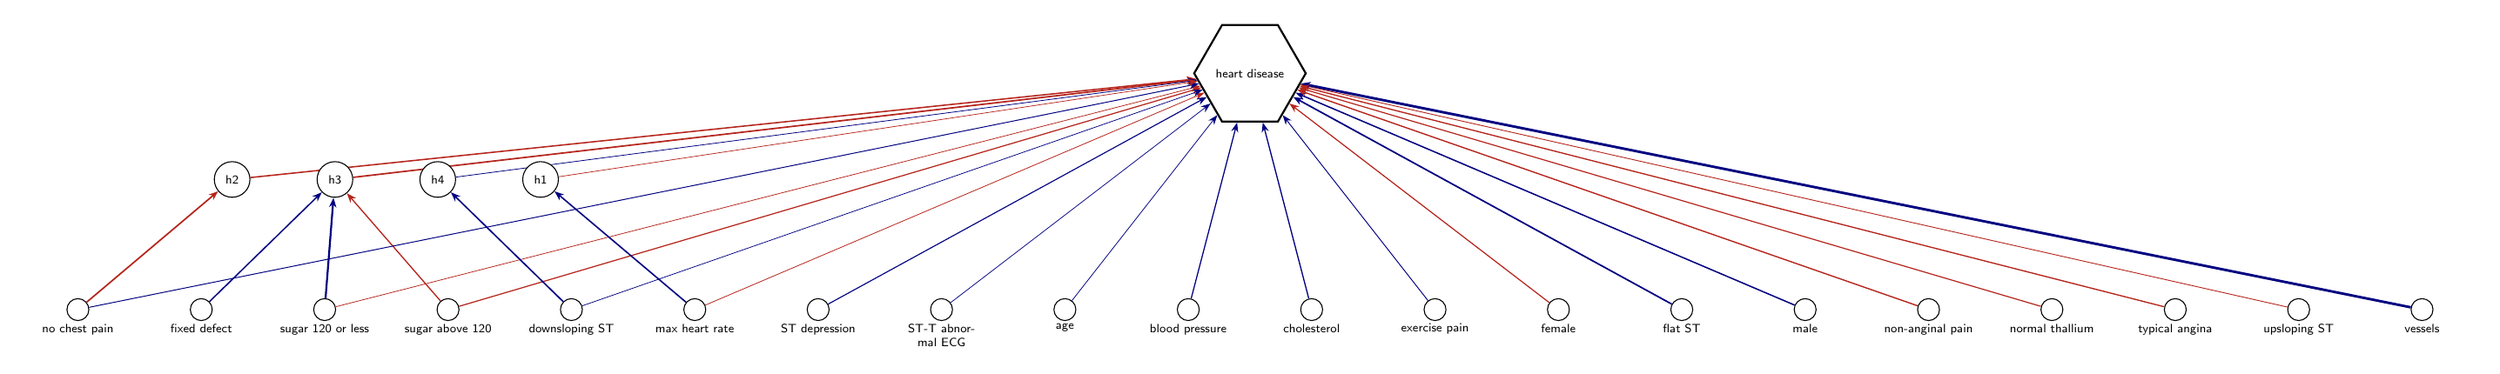
\begin{tikzpicture}[
  font=\sffamily\scriptsize, >={Stealth[length=1.4mm]},
  inp/.style={draw, circle, fill=white, minimum size=3.2mm, inner sep=0pt},
  hid/.style={draw, circle, fill=white, minimum size=5.2mm, inner sep=0.5pt, font=\sffamily\tiny},
  exitbox/.style={draw, thick, rectangle, fill=white, align=center, text width=17mm, minimum height=5mm, inner sep=1.5pt, font=\sffamily\tiny},
  sumbox/.style={draw, thick, dashed, rectangle, fill=white, align=center, text width=17mm, minimum height=5mm, inner sep=1.5pt, font=\sffamily\tiny},
  outp/.style={draw, thick, regular polygon, regular polygon sides=6, fill=white, minimum size=10mm, inner sep=0pt, font=\sffamily\tiny, align=center},
  stub/.style={draw, dashed, rounded corners=2pt, fill=white, align=center, inner sep=2pt, font=\sffamily\tiny, text width=15mm},
  inlab/.style={font=\sffamily\tiny, align=center, text width=15mm, inner sep=1pt, fill=white, fill opacity=0.8, text opacity=1},
  wpos/.style={draw=NavyBlue}, wneg/.style={draw=BrickRed}, wagg/.style={draw=black!45, line width=1.2pt},
  wmix/.style={draw=Plum},
]
\node[inp] (ninxxage) at (14.4,0.0) {};
\path (ninxxage.south) node[inlab, anchor=north] (labninxxage) {age};
\node[inp] (ninxxfbsx0) at (3.6,0.0) {};
\path (ninxxfbsx0.south) node[inlab, anchor=north] (labninxxfbsx0) {sugar 120 or less};
\node[inp] (ninxxfbsx1) at (5.4,0.0) {};
\path (ninxxfbsx1.south) node[inlab, anchor=north] (labninxxfbsx1) {sugar above 120};
\node[inp] (ninxxrestecgx1) at (12.6,0.0) {};
\path (ninxxrestecgx1.south) node[inlab, anchor=north] (labninxxrestecgx1) {ST-T abnormal ECG};
\node[inp] (ninxxthalach) at (9.0,0.0) {};
\path (ninxxthalach.south) node[inlab, anchor=north] (labninxxthalach) {max heart rate};
\node[inp] (ninxxexangx1) at (19.8,0.0) {};
\path (ninxxexangx1.south) node[inlab, anchor=north] (labninxxexangx1) {exercise pain};
\node[inp] (ninxxoldpeak) at (10.8,0.0) {};
\path (ninxxoldpeak.south) node[inlab, anchor=north] (labninxxoldpeak) {ST depression};
\node[inp] (ninxxslopex1) at (32.4,0.0) {};
\path (ninxxslopex1.south) node[inlab, anchor=north] (labninxxslopex1) {upsloping ST};
\node[inp] (ninxxsexx0) at (21.6,0.0) {};
\path (ninxxsexx0.south) node[inlab, anchor=north] (labninxxsexx0) {female};
\node[inp] (ninxxslopex2) at (23.4,0.0) {};
\path (ninxxslopex2.south) node[inlab, anchor=north] (labninxxslopex2) {flat ST};
\node[inp] (ninxxslopex3) at (7.2,0.0) {};
\path (ninxxslopex3.south) node[inlab, anchor=north] (labninxxslopex3) {downsloping ST};
\node[inp] (ninxxca) at (34.2,0.0) {};
\path (ninxxca.south) node[inlab, anchor=north] (labninxxca) {vessels};
\node[inp] (ninxxthalx3) at (28.8,0.0) {};
\path (ninxxthalx3.south) node[inlab, anchor=north] (labninxxthalx3) {normal thallium};
\node[inp] (ninxxthalx6) at (1.8,0.0) {};
\path (ninxxthalx6.south) node[inlab, anchor=north] (labninxxthalx6) {fixed defect};
\node[inp] (ninxxsexx1) at (25.2,0.0) {};
\path (ninxxsexx1.south) node[inlab, anchor=north] (labninxxsexx1) {male};
\node[inp] (ninxxcpx1) at (30.6,0.0) {};
\path (ninxxcpx1.south) node[inlab, anchor=north] (labninxxcpx1) {typical angina};
\node[inp] (ninxxcpx3) at (27.0,0.0) {};
\path (ninxxcpx3.south) node[inlab, anchor=north] (labninxxcpx3) {non-anginal pain};
\node[inp] (ninxxcpx4) at (0.0,0.0) {};
\path (ninxxcpx4.south) node[inlab, anchor=north] (labninxxcpx4) {no chest pain};
\node[inp] (ninxxtrestbps) at (16.2,0.0) {};
\path (ninxxtrestbps.south) node[inlab, anchor=north] (labninxxtrestbps) {blood pressure};
\node[inp] (ninxxchol) at (18.0,0.0) {};
\path (ninxxchol.south) node[inlab, anchor=north] (labninxxchol) {cholesterol};
\node[outp] (n0) at (17.1,3.45) {heart disease};
\node[hid] (n1754) at (2.25,1.9) {h2};
\node[hid] (n2065) at (3.75,1.9) {h3};
\node[hid] (n3504) at (5.25,1.9) {h4};
\node[hid] (n707) at (6.75,1.9) {h1};
\begin{scope}[on background layer]
\draw[->, wpos, line width=0.28pt] (ninxxage) -- (n0);
\draw[->, wneg, line width=0.28pt] (ninxxfbsx0) -- (n0);
\draw[->, wpos, line width=0.80pt] (ninxxfbsx0) -- (n2065);
\draw[->, wneg, line width=0.45pt] (ninxxfbsx1) -- (n0);
\draw[->, wneg, line width=0.49pt] (ninxxfbsx1) -- (n2065);
\draw[->, wpos, line width=0.27pt] (ninxxrestecgx1) -- (n0);
\draw[->, wneg, line width=0.29pt] (ninxxthalach) -- (n0);
\draw[->, wpos, line width=0.59pt] (ninxxthalach) -- (n707);
\draw[->, wpos, line width=0.35pt] (ninxxexangx1) -- (n0);
\draw[->, wpos, line width=0.42pt] (ninxxoldpeak) -- (n0);
\draw[->, wneg, line width=0.33pt] (ninxxslopex1) -- (n0);
\draw[->, wneg, line width=0.45pt] (ninxxsexx0) -- (n0);
\draw[->, wpos, line width=0.64pt] (ninxxslopex2) -- (n0);
\draw[->, wpos, line width=0.27pt] (ninxxslopex3) -- (n0);
\draw[->, wpos, line width=0.60pt] (ninxxslopex3) -- (n3504);
\draw[->, wpos, line width=1.04pt] (ninxxca) -- (n0);
\draw[->, wneg, line width=0.44pt] (ninxxthalx3) -- (n0);
\draw[->, wpos, line width=0.56pt] (ninxxthalx6) -- (n2065);
\draw[->, wpos, line width=0.56pt] (ninxxsexx1) -- (n0);
\draw[->, wneg, line width=0.49pt] (ninxxcpx1) -- (n0);
\draw[->, wneg, line width=0.51pt] (ninxxcpx3) -- (n0);
\draw[->, wpos, line width=0.36pt] (ninxxcpx4) -- (n0);
\draw[->, wneg, line width=0.63pt] (ninxxcpx4) -- (n1754);
\draw[->, wpos, line width=0.46pt] (ninxxtrestbps) -- (n0);
\draw[->, wpos, line width=0.48pt] (ninxxchol) -- (n0);
\draw[->, wneg, line width=0.56pt] (n1754) -- (n0);
\draw[->, wneg, line width=0.63pt] (n2065) -- (n0);
\draw[->, wpos, line width=0.29pt] (n3504) -- (n0);
\draw[->, wneg, line width=0.27pt] (n707) -- (n0);
\end{scope}
\end{tikzpicture}}%
\caption{The network as trained, before any explanation, in full. Blue: positive weight (raises the score); red: negative weight (lowers it); thicker: larger weight. Orange outline and up arrow: raises the final prediction; teal and down arrow: lowers it; grey and double arrow: depends. Not used (no connection): atypical angina, normal ECG, LVH on ECG, no exercise pain, thallium code 4, reversible defect.}
\label{fig:hearts4c1:raw}
\end{figure}
\end{landscape}
\end{drafted}
\clearpage
\end{document}
